% Thesis class does bad things to figure float, mostly because of the double
% spacing. So save off the kernel version of float spacing for reinstatement.
\makeatletter
\let\kernel@xfloat\@xfloat
\makeatother

% Use the class supplied by the University of Calgary
\documentclass[12pt]{ucalgthes1}

% External references
\usepackage[letterpaper,top=1in, bottom= 1in, left= 1in, right= 1in]{geometry}
\usepackage{hyperref}
\usepackage[all]{hypcap}
\usepackage{mathptmx}
\usepackage{ucs}
\usepackage[utf8x]{inputenc}
\usepackage{amsmath}
\usepackage{amssymb}
\usepackage{amsthm}
\usepackage[retainorgcmds]{IEEEtrantools}
\usepackage{mathrsfs}
\usepackage[canadian]{babel}
\usepackage{bbm}
\usepackage{listings}
\usepackage[usenames,dvipsnames]{xcolor}

% Syntax highlighting for julia
% Julia language highlighting
\lstdefinelanguage{Julia}
{
	keywordsprefix=\@,
	morekeywords={abstract,break,case,catch,const,continue,do,else,elseif,end,
			export,false,for,function,immutable,import,importall,if,in,macro,module,
			otherwise,quote,return,switch,true,try,type,typealias,using,while,begin,
			exit,whos,edit,load,is,isa,isequal,typeof,tuple,ntuple,uid,hash,finalizer,
			convert,promote,subtype,typemin,typemax,realmin,realmax,sizeof,eps,
			promote_type,method_exists,applicable,invoke,dlopen,dlsym,system,error,
			throw,assert,new,Inf,Nan,pi,im,let,bitstype,ccall,baremodule,local,global,
			Bool,Int,Int8,Int16,Int32,Int64,Uint,Uint8,Uint16,Uint32,Uint64,Float32,
			Float64,Complex64,Complex128,Any,Nothing,None,Void},
	sensitive=true,
	alsoother={$},
	morecomment=[l]\#,
	morecomment=[n]{\#=}{=\#},
	morestring=[s]{"}{"},
	morestring=[m]{'}{'},
}[keywords,comments,strings]

\lstset{
	language         = Julia,
	basicstyle       = \ttfamily,
	numbers          = left, 
	numberstyle      = \small\ttfamily\color{Gray},
	keywordstyle     = \bfseries\color{blue},
	stringstyle      = \color{Maroon},
	commentstyle     = \color{ForestGreen},
	showstringspaces = false,     
	breaklines       = true,    
	tabsize          = 2,
	lineskip         = -1.5pt,
	extendedchars    = true,
	captionpos       = b
}

% To get Tikz and PGF to work we reinstate the original float
\makeatletter
\def\@xfloat#1[#2]{
        \kernel@xfloat#1[#2]%
        \def\baselinestretch{1}%
        \@normalsize \normalsize
}
\makeatother

% We know return to our originally scheduled programming
\usepackage{pgf}
\usepackage{tikz}

% For the Markov chain diagrams
\usetikzlibrary{arrows,automata}

% Static definitions
\title{The Application of Lie Theory to Markov Processes\\ \bigskip
Computation of the Maximum Likelihood Estimator of the Generator of Continuous 
Time Homogeneous Markov Processes from Stopped Random Variables}
\author{Aaron Geoffrey Sheldon}
\thesisyear{2016}
\thesis{project}
\newcommand{\thesistitle}{The Application of Lie Theory to Markov Processes}
\monthname{August}
\dept{GRADUATE PROGRAM IN "Statistics"}
\degree{"Masters of Science"}

% Mathematical elements
\newtheorem{theorem}{Theorem}
\newtheorem{corollary}{Corollary}
\newtheorem{lemma}{Lemma}
\theoremstyle{definition}\newtheorem{definition}{Definition}
\renewcommand{\IEEEproofindentspace}{0em}
\renewcommand{\IEEEQED}{\IEEEQEDopen}
\interdisplaylinepenalty=0

% Start of main
\begin{document}
	\pagenumbering{gobble}%wierd hack to prevent hyperref warnings due to numbering of the title page
	\makethesistitle
	\pagenumbering{roman}
	\setcounter{page}{2}

%%%%%%%%%%%%%%%%%%%%%%%%%%%%%%%%%%%%%%%%%%%%%%%%%%%%%%%%%%%%%%%%%%%%%%%%%%%%%%%%
%\chapter*{UNIVERSITY OF CALGARY \\ FACULTY OF GRADUATE STUDIES}
%\thispagestyle{empty}
%The undersigned certify that they have read, and recommend
%to the Faculty of Graduate Studies for acceptance, a \Thesis\ entitled
%``\thesistitle'' submitted by \Author\
%in partial fulfillment of the requirements for the degree of
%\Degree.\\
%
%                 Substitute  List of Examiners
%
%\begin{signing}{Department of Academic Computing}
%\signline
%Chairman, Dr.~John D.~Doe \\
%Department of Academic Computing \\
%Services  \\
%\signline
%Chairman, Dr.~John D.~Doe \\
%Department of Academic Computing \\
%Services  \\
%\signline
%Chairman, Dr.~John D.~Doe \\
%Department of Academic Computing \\
%Services  \\
%\signline
%Chairman, Dr.~John D.~Doe \\
%Department of Academic Computing \\
%Services  \\
%\newsigncolumn         use this command to start a new column if necessary
%\newsigncolumn
%\signline
%Chairman, Dr.~John D.~Doe \\
%Department of Academic Computing \\
%Services  \\
%\signline
%Dr.~Jane Smith \\
%Department of Academic Computing  \\

%\signline
%Dr.~A.~B.~Brown \\
%Department of Academic Computing  \\
%\end{signing}
%%%%%%%%%%%%%%%%%%%%%%%%%%%%%%%%%%%%%%%%%%%%%%%%%%%%%%%%%%%%%%%%%%%%%%%%%%%%%%%%

	% Abstract
	\newpage
	\phantomsection
	\altchapter{\bf{Abstract}}
	Individually the probability theory of stochastic processes and Lie theory 
	have been highly productive fields of investigation for more than a century; 
	yet they remain ripe for cross pollination. In particular, the application of 
	algebraic and analytic results from Lie theory can yield novel computational 
	methods for the estimation of generators of continuous time homogeneous Markov 
	processes on finite state spaces. In this project we derive the minimal Lie 
	algebra that contains the generators of continuous time homogeneous Markov 
	processes on finite state spaces, and then using the guarantees of algebraic 
	and analytic closure construct a Newton-Raphson algorithm for maximum 
	likelihood estimation of the generator of a continuous time homogeneous Markov 
	process on a finite state space from stopped random variables using P\'ade 
	approximations for Taylor series expressions of the first and second order 
	derivatives of the exponential map.

	% Acknowledgements
	\newpage
	\phantomsection
	\altchapter{\bf{Acknowledgements}}
	First and foremost is my love and gratitude to my loving family; who 
	withstood the long stretches of my physical presence, but mental absence while 
	I developed, and explored the mathematical geography I describe in this 
	report.
	
	Second, I am deeply appreciative of my supervisor who has had the 
	extraordinary patience to survive the many years of rumination it took for me 
	to develop the meager ideas expressed in this report.

	% Contents listings
	\begin{singlespace}
		\newpage
		\phantomsection
		\tableofcontents
		\pagestyle{plain}
		\newpage
		\phantomsection
		\listoftables
		\pagestyle{plain}
		\newpage
		\phantomsection
		\listoffigures
		\pagestyle{plain}
		\clearpage
		\clearpage
	\end{singlespace}
	\newpage
	\phantomsection
	\chapter*{\bf{List of Symbols, Abbreviations and Nomenclature}\hfill} 
	\addcontentsline{toc}{chapter}{List of Symbols}
	\listofsymbols
	\pagestyle{plain}
	\clearpage
	\pagenumbering{arabic}

	% Content of project
	\chapter{Introduction}
\section{Motivation}
Markov processes are a central subject of study in probability theory, and are a rich source
of distributions for parameter estimation in statistics\cite{billingsley_probability_1995,rogers_diffusions_2000,rogers_diffusions_2000-1}.
They have applications in diverse disciplines ranging through the physical and life
sciences, including operations research, chemical process engineering, queuing theory,
communications theory, natural language processing, finance, and machine learning. Under
mild assumptions and constraints Markov processes offer tractable, and even closed form 
models; that can be reasoned about using physical heuristic analogies, and intuitive
phenomenological interpretations. To varying degrees of rigor, methods for both simulation,
and parameter estimation have been developed for many types of observed random and
pseudo-random processes such as the syntax of sentences, disease states, cancer survival,
epidemiology, and demographics. To apply Markov process a number of simplifying assumptions
are made, including discretization of time and state spaces, homogeneity of the process, and
restrictions of the allowed transitions. The simplifications have resulted in models such as
phase type distributions, branching processes, birth-death processes, and hidden Markov
models.

State of the art computational methods are focused on maximum likelihood parameter
estimation by expectation maximization of hidden Markov Models; which assumes a finite state
space obscured by random noise, with discrete homogeneous time steps, and all times of
transitions being observed. The discretization of time allows for the time evolution of
transition probabilities to be explicitly parameterized through matrix multiplication. The
discrete time construction of hidden Markov models is successfully exploited by the
Baum-Welch, Viterbi, and forward-backward algorithms to estimate parameters.

In contrast continuous time homogeneous Markov processes on a finite state space are more
naturally parameterized through the generator, because the time evolution is represented
through matrix exponentiation. Unfortunately parameterization of the generators of Markov
processes, in more than four states, does not, in general, yield tractable closed form
transition probabilities. This is because any explicit formulation of the transition
probabilities from the generator would require solving the characteristic polynomial of the
generator, which is not generally possible in dimensions greater than four. Yet
computational approximations of the matrix exponential have been well developed, with
methods to compute the gradient receiving recent attention. The focus of this recent
research has been on computing the condition number of numerical problems, as a measure of 
convergence, and stability of the numerical solutions\cite{al-mohy_computing_2009}.

Given a computational method to calculate the matrix exponential, it's gradient, and
Hessian, an application of the chain rule then allows for the computation of maximum
likelihood estimates of any differentiable parameterization of the generators of a
continuous time homogeneous Markov process on a finite state space. Of particular interest
in such a method are stopped statistics, like the first hitting times of transitions from a
fixed source state to a fixed target state. As such this work extends the current
computational methods to include the Hessian of the matrix exponential; and further develops
an alternate direct computation of the gradient of the matrix exponential.

Throughout this work we will attempt to conform to a simplified version of Lamport's guide
to structuring, and presenting proofs\cite{lamport_how_2012}.
\section{Overview}
The Chapman-Kolmogorov equation asserts that every Markov transition probability can be 
represented by a suitable choice of invertible bounded linear operator, that has at least
one Eigen vector with a unit Eigen value. Conversely any choice of invertible bounded linear 
operator, with at least one Eigen vector with a unit Eigen value, can generate a Markov 
transition probability. This characterization of Markov transition probabilities through an
equivalence with invertible bounded linear operators is so intrinsic to Markov processes
that it nearly serves as the definition of a Markov process \cite{rogers_diffusions_2000}.
For a particular Markov process these transitions will form a path through a semi-group.
This semi-group always resides within a Lie group, and thus the generators of the semi-group
reside in the associated Lie algebra. In contrast to the usual analysis of Markov transition
probabilities using resolvents, in the Lie theoretic approach the most general formulation
begins with a continuous path $G_t$ through a Lie algebra on a space of bounded linear
operators. The Markov transition probabilities then arise from the exponential map of the 
Lie algebra to the Lie group. 
\footnote{Usually the linear operators are over some form of $\mathscr{L}^1 \bigcap \mathscr{L}^2$ space of distributions.}
\begin{IEEEeqnarray*}{rCl}
	\mathbb{E}\left[X_{t+\Delta t} \left\| X_{t} \right.\right]
		& = & \left\langle X_{t}, \exp\left(\int_t^{t+\Delta t} G_s ds \right) X_{t+\Delta t} \right\rangle
\end{IEEEeqnarray*}
Knowledge of the stochastic Lie group and algebra provides concrete, and exploitable 
guarantees on the analytic and algebraic properties of the semi-group. For example the
following matrix parameterization
\begin{IEEEeqnarray*}{rCl}
	M_t
		& = & \begin{bmatrix}
			e^{-t} & 1 - e^{-t} \\
			1 - e^{-t} & e^{-t}
		\end{bmatrix}
\end{IEEEeqnarray*}
is a valid stochastic matrix, as $M_t \hat{\mathbbm{1}} = \hat{\mathbbm{1}}$
for all $t \ge 1$. But it is not a Markov process because at $t = \ln 2$ the $\det M_t = 0$,
so that the dual vector $\left[-1,1\right]$ representing the parity statistic on a two state
process vanishes
\begin{IEEEeqnarray*}{rCl}
	\left[-1,1\right] M_t
		& = & \left[-1,1\right]
			\begin{bmatrix}
				e^{-t} & 1 - e^{-t} \\
				1 - e^{-t} & e^{-t}
			\end{bmatrix}\\
		& = & 0
\end{IEEEeqnarray*}
In the context of Lie theory, the path $t$ is not continuous in the Lie algebra.

From the perspective of Lie theory, classical parameter estimation of Markov processes has
been a manifold first approach; starting with an explicit construction of an extrinsic
smooth coordinate chart (parameterization) on a neighborhood of the sub-manifold to which
the generators belong, and only then looking for computational simplifications and
solutions. As hinted to in the previous section, we will proceed with an algebra first
approach; developing the intrinsic algebraic structure of the generators of the Lie algebra,
and then exploiting the chain rule to carry out computations in specific parameterizations.

The second chapter establishes the algebraic and analytic closure properties necessary for 
chapter three, and establishes the notation used throughout all the following chapters.
Chapter two has a secondary role in helping to develop the physical intuition for the 
stochastic Lie group needed to work through the derivatives and approximations of chapter 
three. However, the work on computing the logarithms of permutations can be set aside, as 
the material was developed to gain a fuller understanding of the structure of the stochastic 
Lie algebra; and to highlight, through the explicit construction of examples, the
non-trivial degeneracy of the branches of the matrix logarithm.

The third chapter reviews the definition for the gradient of exponential map, and continues
on to derive a Pad\'{e} approximation of the gradient of the exponential map. An analytic
form for the Hessian of the exponential map is then developed, followed by an algorithm that
to calculate the Hessian of the exponential map. The Hessian approximation algorithm
involves a combination of a Pad\'{e} approximation of a linear term, and a novel recursive 
calculation of a bilinear non-commutative perturbation to the Hessian.

The fourth chapter seeks to illustrate the material developed in the preceding two chapters.
First the cumulative distribution of the stopped statistic of first hitting times is recast 
in the stochastic Lie algebra developed in chapter two. These results are then put to use in
developing a model for an aging process; which is a finite state reversible birth-death
process. The chapter concludes by laying out the algorithms to calculate the gradient and
Hessian of the log-likelihood of the aging process, and hence a Newton-Raphson method for
maximization.

Finally, the fifth chapter concludes with summarizing remarks, and a discussion of the
direction for further investigation.
	\chapter{The Lie Algebra of Markov Process Generators}
\section{Stochastic Matrices}
\subsection{Preliminaries}
The classical Lie algebras of physics, like the infinitesimal symmetries of the special
unitary algebra $\mathfrak{su}(n)$, are defined with respect to invariants of a Banach
algebra, such as the matrix invariants of the determinant, trace, or norm. In contrast,
stochastic matrices are always characterized with respect to a choice of a specific single
subspace spanned by a vector of unit norm. For reasons that will become clear later, we will
denote this characterizing unit vector by $\hat{\mathbbm{1}}$
\footnote{For the remainder of the text vectors will be denoted with the over arrow $\vec{v}$, and vectors of unit norm will be denoted with the hat $\hat{u}$; so that $\left\| \hat{u} \right\| = 1$}. In the next two sections we 
will provide an explicit construction and characterization of the Lie algebra of stochastic 
matrices, building on the original work of Johnson \cite{johnson_markov-type_1985} and
distilling the recent works of Sumner et al. \cite{sumner_lie_2012,fernandez-sanchez_lie_2012} 
Mourad \cite{mourad_lie-theoretic_2004} and Chruściński et al. \cite{chruscinski_pseudo-stochastic_2015}.

The common approach to stochastic matrices begins with the restriction that a matrix, $A$,
has non-negative entries with respect to the standard orthonormal basis for the vector
space on which it acts; namely $\left\langle\hat{e}_i,A \hat{e}_j\right\rangle \ge 0$ for 
all $i,j$. In addition to allowing for singular matrices, this poses an immediate obstacle
to the necessary closure with respect to matrix inversion required for matrix groups; as the
inverse of a stochastic matrix need not have non-negative entries with respect to the
standard orthonormal basis. 

For the moment we will set aside the restriction that the entries be non-negative, and
instead begin with a generalization of fixed row sums to abstract linear operators. We will
show that this generalization is preserved by operator inversion, and then develop an
orthonormal basis from which matrix representations of the abstract linear operators can be
constructed with non-negative entries. In essence tackling the problem from the reverse
direction, starting with an abstract generalization of the idea of fixed row sums, and then 
specifying matrices with non-negative entries with respect to a constructed orthonormal
basis.
\begin{definition}
	A bounded linear operator $A$ on a finite dimensional Hilbert space is stochastic with
	respect to the unit vector $\hat{\mathbbm{1}}$ if $A \hat{\mathbbm{1}} = \hat{\mathbbm{1}}$
\end{definition}
Note that this definition does not stipulate any conditions on non-singularity, and thus
includes, as representations of the linear operators, all the matrices in the convex
polytope of stochastic matrices. For an $n$ dimensional vector space the vector $\vec{\mathbbm{1}} = \sqrt{n} \hat{\mathbbm{1}}$
acts as the row sum operator on bounded linear operators stochastic with respect to $\hat{\mathbbm{1}}$. 
We will make this claim more precise after we dispense with a few more foundational
definitions.
\begin{definition}
	Let $St(\hat{\mathbbm{1}})$ denote the stochastic Lie group of invertible bounded linear
	operators stochastic with respect to $\hat{\mathbbm{1}}$.
\end{definition}
It is tempting to view the name stochastic Lie group as a bait and switch, or at least an
abuse of the terminology, given we have removed the usual convex polytope of stochastic
matrices and replaced it with a group of invertible bounded linear operators with a common
eigenvector $\hat{\mathbbm{1}}$. Previous authors have denoted the convex polytope of
stochastic matrices as the stochastic semi-group, and the group of invertible matrices as
the pseudo-stochastic Lie group. One could even consider incorporating Markov into the name,
in reference to the fact that the transition matrices of a continuous time homogeneous
Markov process on a finite-state space are by definition invertible, and have common
eigenvector $\hat{\mathbbm{1}}$. However the suffix of Lie group in the name connotes both
sufficient additional restrictions to make the name distinct, and still allows for an
indication of a relationship with the original concept. Of course, this definition
immediately necessitates a proof of the claim embedded in the definition.
\begin{lemma}
	$St(\hat{\mathbbm{1}})$ is a Lie group
\end{lemma}
\begin{IEEEproof}
	We proceed by working mechanistically through the Lie group axioms \cite{hall_lie_2004}.
	\begin{enumerate}
		\item The identity element $I$ is in $St(\hat{\mathbbm{1}})$. Clearly $I$ is invertible
		and $I \hat{\mathbbm{1}} = \hat{\mathbbm{1}}$.
		\item If $A,B \in St(\hat{\mathbbm{1}})$ then $AB \in St(\hat{\mathbbm{1}})$. This
		follows from the computation $AB \hat{\mathbbm{1}} = A \hat{\mathbbm{1}} = \hat{\mathbbm{1}}$.
		\item If $A \in St(\hat{\mathbbm{1}})$ then $A^{-1} \in St(\hat{\mathbbm{1}})$.
		Recognize that $A \hat{\mathbbm{1}} = \hat{\mathbbm{1}}$ implies $\hat{\mathbbm{1}} = A^{-1} A \hat{\mathbbm{1}} = A^{-1} \hat{\mathbbm{1}}$.
		\item Associativity follows from $St(\hat{\mathbbm{1}})$ being a subgroup of $GL\left(n\right)$.
		\item Finally, we need to prove that is $St(\hat{\mathbbm{1}})$ closed within $GL\left(n\right)$.
		Consider a sequence $A_n \in St(\hat{\mathbbm{1}})$ that converges to $A$, then $\hat{\mathbbm{1}} = A_n \hat{\mathbbm{1}} \rightarrow A \hat{\mathbbm{1}}$. 
		Now if $A$ is invertible then we are done, and if $A$ is not invertible then $A \notin GL\left(n\right)$,
		again satisfying closure within $GL\left(n\right)$.\hfill\IEEEQEDhere
	\end{enumerate}
\end{IEEEproof}
That $St(\hat{\mathbbm{1}})$ is a proper Lie group implies that it must be infinitesimal
generated by elements of a Lie algebra.
\begin{definition}
	Let $\mathfrak{st}(\hat{\mathbbm{1}})$ denote the stochastic Lie algebra of $St(\hat{\mathbbm{1}})$
\end{definition}
By infinitesimally generated we mean that every element of $St(\hat{\mathbbm{1}})$ is the
exponential map of at least one element in $\mathfrak{st}(\hat{\mathbbm{1}})$. We can fully
characterize this algebra as the set of bounded linear operators such that $\hat{\mathbbm{1}}$
is in the kernel of each operator.
\begin{lemma}
	The algebra $\mathfrak{st}(\hat{\mathbbm{1}})$ is exactly the set of all bounded linear
	operators with $\hat{\mathbbm{1}}$ in their kernel.
\end{lemma}
\begin{IEEEproof}
	Working through the forward and backward inclusions we have
	\begin{enumerate}
		\item Suppose $A \hat{\mathbbm{1}} = 0$ then from the definition of the exponential map
		we have:
		\begin{IEEEeqnarray*}{rCl}
			\exp\left(A\right) \hat{\mathbbm{1}}
				& = & \sum_{n=0}^{\infty} \frac{1}{n!} A^n \hat{\mathbbm{1}}\\
				& = & \hat{\mathbbm{1}} + \sum_{n=1}^{\infty} \frac{1}{n!} 0\\
				& = & \hat{\mathbbm{1}}
		\end{IEEEeqnarray*}
		Thus $\exp\left(A\right) \in St(\hat{\mathbbm{1}})$ implying that $A \in \mathfrak{st}(\hat{\mathbbm{1}})$
		\item Now proceeding with the reverse assumption, that $A \in \mathfrak{st}(\hat{\mathbbm{1}})$.
		For all $t \in \mathbb{R}$ we have $\exp\left(tA\right) \hat{\mathbbm{1}} = \hat{\mathbbm{1}}$.
		Differentiation with respect to $t$ and evaluation at $t = 0$ yields
		\begin{IEEEeqnarray*}{+rCl+x*}
			0 & = & \left. \frac{d}{dt} \hat{\mathbbm{1}} \right|_{t=0}\\
				& = & \left. \frac{d}{dt} \exp\left(tA\right) \hat{\mathbbm{1}} \right|_{t=0}\\
				& = & \left. \exp\left(tA\right) A \hat{\mathbbm{1}} \right|_{t=0}\\
				& = & A \hat{\mathbbm{1}} & \IEEEQEDhere
		\end{IEEEeqnarray*}
	\end{enumerate}
\end{IEEEproof}
The following chapter will hinge on taking the derivatives of smooth parameterizations $X : \mathbb{R}^k \mapsto \mathfrak{st}(\hat{\mathbbm{1}})$. 
The principle role of this chapter is to assure ourselves that we will not differentiate
ourselves out of $\mathfrak{st}(\hat{\mathbbm{1}})$. The next corollary nicely provides just
such an assurance:
\begin{corollary}
	The tangent space $T\mathfrak{st}(\hat{\mathbbm{1}}) = \mathfrak{st}(\hat{\mathbbm{1}})$
\end{corollary}
\begin{IEEEproof}
	The proof is complementary to the preceding lemma and moves through each direction of
	inclusion:
	\begin{enumerate}
		\item To show that $\mathfrak{st}(\hat{\mathbbm{1}})\subseteq T\mathfrak{st}(\hat{\mathbbm{1}})$
		consider $X\left(x\right) = x X_0$ where $x$ is a scalar parameter and $X_0 \in \mathfrak{st}(\hat{\mathbbm{1}})$
		\item Clearly $X\left(x\right) \in \mathfrak{st}(\hat{\mathbbm{1}})$
		\item Furthermore the tangent $\frac{\partial}{\partial x} X\left(x\right) = X_0 \in \mathfrak{st}(\hat{\mathbbm{1}})$
		\item Now to show that $T \mathfrak{st}(\hat{\mathbbm{1}}) \subseteq \mathfrak{st}(\hat{\mathbbm{1}})$
		we start with an arbitrary smooth parameterization $X\left(x\right) : \mathbb{R}^k \mapsto \mathfrak{st}(\hat{\mathbbm{1}})$
		\item Using the same trick of differentiation we have
		\begin{IEEEeqnarray*}{+rCl+x*}
			0 & = & \frac{\partial}{\partial x} 0\\
				& = & \frac{\partial}{\partial x} \left( X\left(x\right) \hat{\mathbbm{1}}\right)\\
				& = & \left(\frac{\partial}{\partial x} X\left(x\right)\right) \hat{\mathbbm{1}} & \IEEEQEDhere
		\end{IEEEeqnarray*}
	\end{enumerate}
\end{IEEEproof}
Clearly the tangent space to a normed vector space is the normed vector space. After all one
can just choose a fixed basis and then differentiate the individual smoothly parameterized
in projections. However, the proof of the preceding corollary was constructed to explicitly
connect algebraic closure and differentiation, with the norm implicitly used in the
differentiation. The proof further illustrates the intuition that any increase in a
particular matrix element has to be compensated for by an equal decrease in some other
matrix elements.
\subsection{Canonical Generators}
Over an $n$ dimensional vector space, the condition on a matrix $A$ that $A \hat{\mathbbm{1}} = 0$
places $n$ constraints on the $n^2$ dimensions of $A$. This leaves $n^2 - n$ free dimensions
on $\mathfrak{st}(\hat{\mathbbm{1}})$, when considered as a vector space. This hints that we
can construct a generator of $\mathfrak{st}(\hat{\mathbbm{1}})$ from order pairs of basis
elements $\hat{e}_i$ for the vector space of $\hat{\mathbbm{1}}$. To see how this is done we
first construct a useful basis for the vector space to which $\hat{\mathbbm{1}}$ is a
member.
\begin{lemma}
	There exists an orthonormal basis $\hat{e}_i$ such that $\left\langle \hat{e}_i, \hat{\mathbbm{1}} \right\rangle = \frac{1}{\sqrt{n}}$
	for all $i$
\end{lemma}
\begin{IEEEproof}
	While a basis with the stipulated properties can be constructed through the Gram-Schmidt
	process, the proof of the existence proceeds by induction.
	\begin{enumerate}
		\item For $n=1$ the desired basis is precisely the trivial set $\left\lbrace \hat{\mathbbm{1}} \right\rbrace$ 
		which satisfies the condition that $\left\langle \hat{\mathbbm{1}}, \hat{\mathbbm{1}} \right\rangle = 1$.
		\item Assume the claim is true for $n$. For $n+1$ pick a unit vector $\hat{e}_{\perp}$
		that is orthogonal to $\hat{\mathbbm{1}}$ and construct the unit vector
		$\hat{e}_{n+1} = \frac{1}{\sqrt{n+1}} \hat{\mathbbm{1}} + \sqrt{\frac{n}{n+1}} \hat{e}_{\perp}$.
		Clearly $\hat{e}_{n+1}$ satisfies the condition $\left\langle \hat{e}_{n+1}, \hat{\mathbbm{1}} \right\rangle = \frac{1}{\sqrt{n+1}}$.
		\item To use the the induction assumption we construct a new row sum unit vector $\hat{\mathbbm{1}}_n = \sqrt{\frac{n+1}{n}}\hat{\mathbbm{1}} - \frac{1}{\sqrt{n}}\hat{e}_{n+1}$ 
		in one dimension lower by projecting onto the subspace orthogonal to $\hat{e}_{n+1}$.
		\item By the induction assumption there exists a basis $\hat{e}_i$ with $i \le n$, such
		that $\left\langle \hat{e}_i, \hat{\mathbbm{1}}_n \right\rangle = \frac{1}{\sqrt{n}}$.
		\item Because $\hat{e}_i$ with $i \le n$ was constructed in the space orthogonal to $\hat{e}_{n+1}$
		it follows that $\left\langle \hat{e}_i, \hat{e}_j \right\rangle = \delta_{ij}$ for all
		$i,j \le n+1 $.
		\item Then using the definitions of $\hat{e}_{n+1}$ and $\hat{\mathbbm{1}}_n$ we can
		calculate the inner product $\left\langle \hat{e}_i, \hat{\mathbbm{1}}_n \right\rangle$
		for $i \le n$
		\begin{IEEEeqnarray*}{rCl}
			\frac{1}{\sqrt{n}}
				& = & \left\langle \hat{e}_i, \hat{\mathbbm{1}}_n \right\rangle\\
				& = & \sqrt{\frac{n+1}{n}} \left\langle \hat{e}_j, \hat{\mathbbm{1}} \right\rangle - \frac{1}{\sqrt{n}} \left\langle \hat{e}_i, \hat{e}_{n+1} \right\rangle\\
				& = & \sqrt{\frac{n+1}{n}} \left\langle \hat{e}_j, \hat{\mathbbm{1}} \right\rangle
		\end{IEEEeqnarray*}
		Inverting the fraction in the equality yields $\left\langle \hat{e}_i, \hat{\mathbbm{1}} \right\rangle = \frac{1}{\sqrt{n+1}}$
		for all $i \le n+1$.\hfill\IEEEQEDhere
	\end{enumerate}
\end{IEEEproof}
As a direct result of the construction of the basis vectors $\hat{e}_i$ we see that $\vec{\mathbbm{1}} = \sum_{i=1}^n \hat{e}_i$.
Thus $\vec{\mathbbm{1}}$ can be interpreted as the row sum vector in basis $\hat{e}_i$.

The constructed basis leads naturally to considering the minimal non-trivial matrices $C_{ij} = \hat{e}_i \otimes \left( \hat{e}_j - \hat{e}_i \right)$,
as holding significance in the structure of $\mathfrak{st}(\hat{\mathbbm{1}})$. These 
matrices are illustrated as state transitions in figure \ref{fig:singlestochastic}. In fact 
this will be the central result of this chapter: that the algebraic closure of the matrices 
$C_{ij}$ is the stochastic Lie algebra $\mathfrak{st}(\hat{\mathbbm{1}})$. To establish this 
result we need a preliminary result that proves the commutators $\left[C_{ij},C_{kl}\right]$ 
are linear combinations of matrices $C_{ij}$.
\begin{lemma}
	\begin{IEEEeqnarray*}{rCl}
		C_{ij}C_{kl} & = &
		\begin{cases}
			- C_{il} & i=k,\\
			C_{il} - C_{ij} & j=k,\\
			0 & \text{otherwise}.
		\end{cases}
	\end{IEEEeqnarray*}
\end{lemma}
\begin{IEEEproof}
	We proceed in two steps; calculating the terms of the products, then simplifying the 
	cases, always assuming $i \neq j$ and $k \neq l$.
	\begin{enumerate}
		\item Term wise computation of the Kronecker products yields
		\begin{IEEEeqnarray*}{rCl}
			C_{ij}C_{kl}
				& = & \hat{e}_i \otimes \left( \hat{e}_j - \hat{e}_i \right) \hat{e}_k \otimes \left( \hat{e}_l - \hat{e}_k \right)\\
				& = & \hat{e}_i \otimes \hat{e}_j \hat{e}_k \otimes \hat{e}_l + \hat{e}_i \otimes \hat{e}_i \hat{e}_k \otimes \hat{e}_k - \hat{e}_i \otimes \hat{e}_j \hat{e}_k \otimes \hat{e}_k - \hat{e}_i \otimes \hat{e}_i \hat{e}_k \otimes \hat{e}_l\\
				& = & \delta_{jk} \hat{e}_i \otimes \hat{e}_l + \delta_{ik} \hat{e}_i \otimes \hat{e}_k - \delta_{jk} \hat{e}_i \otimes \hat{e}_k - \delta_{ik} \hat{e}_i \otimes \hat{e}_l\\
				& = & \left(\delta_{jk} - \delta_{ik} \right) \hat{e}_i \otimes \left( \hat{e}_l - \hat{e}_k \right)
		\end{IEEEeqnarray*}
		\item We work through each case of $\delta_{jk} - \delta_{ik}$, starting with the case $i=k$ 
		\begin{IEEEeqnarray*}{rCl}
			C_{ij}C_{il}
				& = & \left(\delta_{jk} - \delta_{ii} \right) \hat{e}_i \otimes \left( \hat{e}_l - \hat{e}_i \right)\\
				& = & - \hat{e}_i \otimes \left( \hat{e}_l - \hat{e}_i \right)\\
				& = & - C_{il}
		\end{IEEEeqnarray*}
		\item When $j=k$ we have
		\begin{IEEEeqnarray*}{rCl}
			C_{ij}C_{jl}
				& = & \left(\delta_{jj} - \delta_{ij} \right) \hat{e}_i \otimes \left( \hat{e}_l - \hat{e}_j \right)\\
				& = & \hat{e}_i \otimes \left( \hat{e}_l - \hat{e}_j \right)\\
				& = & \hat{e}_i \otimes \left( \hat{e_l} - \hat{e}_i + \hat{e}_i - \hat{e}_j \right)\\
				& = & C_{il} - C_{ij}
		\end{IEEEeqnarray*}
		\item Finally when none of the previous conditions apply
		\begin{IEEEeqnarray*}{+rCl+x*}
			C_{ij}C_{kl}
				& = & \left(\delta_{jk} - \delta_{ik} \right) \hat{e}_i \otimes \left( \hat{e}_l - \hat{e}_k \right)\\
				& = & 0 \cdot \hat{e}_i \otimes \left( \hat{e}_l - \hat{e}_k \right)\\
				& = & 0 & \IEEEQEDhere
		\end{IEEEeqnarray*}
	\end{enumerate}
\end{IEEEproof}
While this result is sufficient to accomplish the central result, it is worth carrying
through with the computation of the structure constants of the generators.
\begin{corollary}
	\begin{IEEEeqnarray*}{rCl}
		\left[C_{ij},C_{kl}\right] & = &
		\begin{cases}
			C_{ij} - C_{il} & i=k,\\
			C_{kj} - C_{ki} & i=l,\\
			C_{il} - C_{ij} & j=k,\\
			0 & \text{otherwise}.
		\end{cases}
	\end{IEEEeqnarray*}
\end{corollary}
\begin{IEEEproof}
	As in the previous lemma we work case wise through the equalities.
	\begin{enumerate}
		\item Starting with $i=k$
		\begin{IEEEeqnarray*}{rCl}
			\left[C_{ij},C_{il}\right]
				& = & C_{ij}C_{il} - C_{il}C_{ij}\\
				& = & C_{ij} - C_{il}
		\end{IEEEeqnarray*}
		\item For $i=l$
		\begin{IEEEeqnarray*}{rCl}
			\left[C_{ij},C_{ki}\right]
				& = & C_{ij}C_{ki} - C_{ki}C_{ij}\\
				& = & C_{kj} - C_{ki}
		\end{IEEEeqnarray*}
		\item For $j=k$
		\begin{IEEEeqnarray*}{rCl}
			\left[C_{ij},C_{jl}\right]
				& = & C_{ij}C_{jl} - C_{jl}C_{ij}\\
				& = & C_{il} - C_{ij}
		\end{IEEEeqnarray*}
		\item When none of the conditions apply
		\begin{IEEEeqnarray*}{+rCl+x*}
			\left[C_{ij},C_{kl}\right]
				& = & C_{ij}C_{kl} - C_{kl}C_{ij}\\
				& = & 0 & \IEEEQEDhere
		\end{IEEEeqnarray*}
	\end{enumerate}
\end{IEEEproof}
We can now proceed with the central result that motivates this chapter.
\begin{theorem}
	The canonical generators of $\mathfrak{st}(\hat{\mathbbm{1}})$ are $C_{ij}$
\end{theorem}
\begin{IEEEproof}
	The previous lemma has established that the products, and thus the commutators, of $C_{ij}$
	are linear in $C_{ij}$. We then have to prove that the smallest algebra that contains $C_{ij}$
	is $\mathfrak{st}(\hat{\mathbbm{1}})$. As thus, it is sufficient to prove that matrices $C_{ij}$
	from a basis for $\mathfrak{st}(\hat{\mathbbm{1}})$. This is because a necessary condition
	for an algebra to contain the matrices $C_{ij}$ is that it must contain all sums of the
	matrices $C_{ij}$. If one could sum their way out of the algebra then it would not be an
	algebra.
	\begin{enumerate}
		\item That $\mathfrak{st}(\hat{\mathbbm{1}})$ is an $n^2-n$ dimensional vector space
		should be clear from the previous discussion. A full formal proof of this claim is found
		through induction on the dimension $n$.
		\item The matrices $C_{ij}$ are in $\mathfrak{st}(\hat{\mathbbm{1}})$. From the 
		definition of the canonical generators
		\begin{IEEEeqnarray*}{rCl}
			C_{ij} \hat{\mathbbm{1}}
				& = & \hat{e}_i \otimes \left( \hat{e}_j - \hat{e}_i \right) \hat{\mathbbm{1}}\\
				& = & \hat{e}_i \left( \left\langle \hat{e}_j, \hat{\mathbbm{1}} \right\rangle - \left\langle \hat{e}_i, \hat{\mathbbm{1}} \right\rangle \right)\\
				& = & \hat{e}_i \left(\frac{1}{\sqrt{n}} - \frac{1}{\sqrt{n}}\right)\\
				& = & 0
		\end{IEEEeqnarray*}
		\item $C_{ij}$ is a set of $n^2-n$ linear independent matrices and so must form a basis
		for all of $\mathfrak{st}(\hat{\mathbbm{1}})$. That there are only $n^2-n$ matrices is
		clear from the fact that $C_{ii} = 0$. While the formal proof of linear independence is
		again found through induction on the dimension $n$.\hfill\IEEEQEDhere
	\end{enumerate}
\end{IEEEproof}
The previous theorem serves as the definition of a set of canonical generators of $\mathfrak{st}(\hat{\mathbbm{1}})$.
It is  important to note that neither the basis $\hat{e}_i$ nor the canonical generators $C_{ij}$
are unique. They are defined only up to rotations orthogonal to the vector $\hat{\mathbbm{1}}$.
Regardless of the choice of basis $\hat{e}_i$, Jacobi's formula implies that if $G = \sum_{i,j} \alpha_{ij} C_{ij}$
then $\det G = \exp\left( \sum_{i,j} \alpha_{ij} \right)$.
\subsection{Vertex Logarithms}
Geometrically fixing a basis $\hat{e}_i$ defines the convex polytope of all matrices, $M$,
stochastic with respect to $\hat{\mathbbm{1}}$ that have nonnegative entries with respect to
$\hat{e}_i$; also designated the convex polytope of singly stochastic matrices. The vertexes 
of the convex polytope of nonnegative stochastic matrices with respect to $\hat{e}_i$ can be
formulated as linear combinations of the generators $C_{ij}$ of $\mathfrak{st}(\hat{\mathbbm{1}})$.
\begin{definition}
	For a function $j(i): \left\lbrace 1,\dots,n \right\rbrace \mapsto S \subseteq \left\lbrace 1,\dots,n \right\rbrace$
	the vertex matrix is given by $V_{j\left(\cdot\right)} = I + \sum_{i=1}^n C_{ij\left(i\right)}$
\end{definition}
Every vertex matrix is uniquely dual to a matrix in $\mathfrak{st}(\hat{\mathbbm{1}})$ 
through the relationship
\begin{IEEEeqnarray*}{rCl}
	V_{j\left(\cdot\right)} - I
		& = & \sum_{i=1}^n \hat{e}_i \otimes \hat{e}_{j\left(i\right)} - \hat{e}_i \otimes \hat{e}_i\\
		& = & C_{j\left(\cdot\right)}
\end{IEEEeqnarray*}
It is important to note that in general the vertex duals $C_{j\left(\cdot\right)}$ in $\mathfrak{st}(\hat{\mathbbm{1}})$
are not the generators, nor logarithms, of the vertexes $V_{j\left(\cdot\right)}$. In fact, 
if there exists $i_1 \ne i_2$ such that $j\left(i_i\right) = j\left(i_2\right)$ then $V_{j\left(\cdot\right)}$
does not have a generator, or logarithm. However, in this situation we will show that $V_{j\left(\cdot\right)}$
is a limit point of the boundary of $\mathfrak{st}(\hat{\mathbbm{1}})$.

For now we need to establish the claim implicit in the definition of the vertex matrices.
\begin{lemma}
	The convex hull of the $n^n$ vertex matrices $V_{j\left(\cdot\right)}$ is the convex
	polytope of nonnegative stochastic matrices with respect to $\hat{e}_i$.
\end{lemma}
\begin{IEEEproof}
	The proof proceeds by showing each direction of inclusion.
	\begin{enumerate}
		\item Starting with the forward inclusion, clearly every $V_{j\left(\cdot\right)}$ 
		belongs to the convex polytope of singly stochastic matrices.
		\item It follows that any convex sum of the vertexes $V_{j\left(\cdot\right)}$ also 
		belongs to the convex polytope of singly stochastic matrices.
		\item In the reverse inclusion, we work analogously to the Birkhoff-von Neumann theorem;
		where starting with a matrix $M$ in the convex polytope of singly stochastic matrices we 
		eliminate nonzero entries from $M$ with convex sums involving $V_{j\left(\cdot\right)}$.
		\item Begin by picking a pair $i,j$ such that $m_{ij} = \left\langle \hat{e}_i, M \hat{e}_j \right\rangle$
		is the smallest $m_{ij} > 0$. Which we can always do because $M \vec{\mathbbm{1}} = \vec{\mathbbm{1}}$.
		If $m_{ij} = 1$ then by definition $M$ is a vertex matrix and we are done.
		\item By the same argument we can pick a function $f^{\left(1\right)}\left(k\right) : \left\lbrace 1,\dots,n \right\rbrace \mapsto S \subseteq \left\lbrace 1,\dots,n \right\rbrace$
		such that $f^{\left(1\right)}\left(i\right)=j$ and $m_{k f^{\left(1\right)}\left(k\right)} \ge m_{ij}$ for all other $k \ne i$.
		\item Letting $M^{\left(0\right)} = M$ we can decompose $M^{\left(1\right)}$ into the 
		convex sum
		\begin{IEEEeqnarray*}{rCl}
			M^{\left(0\right)}
				& = & \left(1 - m_{ij} \right) M^{\left(1\right)} + m_{ij} V_{f^{\left(1\right)}\left(\cdot\right)}
		\end{IEEEeqnarray*}
		It remains then to establish that $M^{\left(1\right)}$ is an element of the convex 
		polytope of singly stochastic matrices.
		\item Checking that $M^{\left(1\right)}$ has $\hat{\mathbbm{1}}$ as an Eigen vector with Eigen value $1$
		\begin{IEEEeqnarray*}{rCl}
			M^{\left(1\right)} \hat{\mathbbm{1}}
				& = & \frac{M^{\left(0\right)}  \hat{\mathbbm{1}} - m_{ij}V_{f^{\left(1\right)}\left(\cdot\right)}  \hat{\mathbbm{1}}}{1 - m_{ij}}\\
				& = & \frac{1 - m_{ij}}{1 - m_{ij}} \hat{\mathbbm{1}}\\
				& = & \hat{\mathbbm{1}}
		\end{IEEEeqnarray*}
		\item We then check to ensure that $\left\langle \hat{e}_k, M^{\left(1\right)} \hat{e}_l \right\rangle > 0$
		for every $k,l$
		\begin{IEEEeqnarray*}{rCl}
			\left\langle \hat{e}_k, M^{\left(1\right)} \hat{e}_l \right\rangle
				&  =  & \frac{\left\langle \hat{e}_k,M^{\left(0\right)} \hat{e}_l\right\rangle -  m_{ij} \left\langle \hat{e}_k, V_{f^{\left(1\right)}\left(\cdot\right)} \hat{e}_l\right\rangle }{1 - m_{ij}}\\
				&  =  & \frac{m_{kl} - m_{ij} \delta_{f\left(k\right)l}}{1 - m_{ij}}\\
				& \ge & 0
		\end{IEEEeqnarray*}
		because $m_{kl} \ge m_{ij}$ for all $k,l$ by construction, and $1 > m_{ij}$; or else we 
		are done.
		\item Next, observe that $\left\langle \hat{e}_i, M^{\left(1\right)} \hat{e}_j \right\rangle = 0$, 
		so that we can carry out finite induction on this process, at most $n^2$ times. 
		\item Finally, the finite induction will generate matrices $M^{\left(t\right)}$ and $V_{f^{\left(t\right)}\left(\cdot\right)}$, 
		proving that $M$ is the convex sum of vertexes $V_{f^{\left(t\right)}\left(\cdot\right)}$.\hfill\IEEEQEDhere
	\end{enumerate}
\end{IEEEproof}
The vertex dual matrices $C_{j\left(\cdot\right)}$ have a powerful commutator algebra. We
start with a calculation of the products of vertex dual matrices.
\begin{corollary}
	$C_{j\left(\cdot\right)} C_{k\left(\cdot\right)} = C_{k\left(j\left(\cdot\right)\right)} - C_{j\left(\cdot\right)} - C_{k\left(\cdot\right)}$
\end{corollary}

\begin{IEEEproof}
	Calculating directly from the definitions
	\begin{IEEEeqnarray*}{+rCl+x*}
		C_{j\left(\cdot\right)} C_{k\left(\cdot\right)}
			& = & \left(\sum_{i=1}^n \hat{e}_i \otimes \hat{e}_{j\left(i\right)} - \hat{e}_i \otimes \hat{e}_i\right) \left(\sum_{i=1}^n \hat{e}_i \otimes \hat{e}_{k\left(i\right)} - \hat{e}_i \otimes \hat{e}_i\right)\\
			& = & \sum_{i=1}^n \hat{e}_i \otimes \hat{e}_{k\left(j\left(i\right)\right)} - \hat{e}_i \otimes \hat{e}_{j\left(i\right)} - \hat{e}_i \otimes \hat{e}_{k\left(i\right)} + \hat{e}_i \otimes \hat{e}_i\\
			& = & C_{k\left(j\left(\cdot\right)\right)} - C_{j\left(\cdot\right)} - C_{k\left(\cdot\right)}\\
			& = & C_{j \circ k \left(\cdot\right)} - C_{j\left(\cdot\right)} - C_{k\left(\cdot\right)} & \IEEEQEDhere
	\end{IEEEeqnarray*}
\end{IEEEproof}
We can state immediately without proof, that the commutators of $C_{j\left(\cdot\right)}$
carry through with the commutation of $j\left(\cdot\right)$ and $k\left(\cdot\right)$.
\begin{corollary}
	$\left[C_{j\left(\cdot\right)}, C_{k\left(\cdot\right)}\right] = C_{k\left(j\left(\cdot\right)\right)} - C_{j\left(k\left(\cdot\right)\right)}$
\end{corollary}
Furthermore, recognizing that $C_{j^0\left(\cdot\right)} = 0$, because $j^0_{\left(i\right)} = i$
for all $i$, we have that the powers of $C_{j\left(\cdot\right)}$ have the binomial form.
\begin{corollary}
	For $n>0$ we have $C_{j\left(\cdot\right)}^n = \sum_{m=0}^n \binom{n}{m} \left(-1\right)^{n-m} C_{j^m\left(\cdot\right)}$
\end{corollary}
\begin{IEEEproof}
	Starting with $n = 1$ we carry through with induction.
	\begin{enumerate}
		\item Explicitly calculating for $n = 1$ we have
		\begin{IEEEeqnarray*}{rCl}
			C_{j\left(\cdot\right)} 
				& = & C_{j\left(\cdot\right)} - C_{j^0\left(\cdot\right)}\\
				& = & \sum_{m=0}^1 \binom{1}{m} \left(-1\right)^{1-m} C_{j^m\left(\cdot\right)}
		\end{IEEEeqnarray*}
		\item Now assume the claim is true for a fixed $n$, setting up the calculation for $n+1$
		we have
		\begin{IEEEeqnarray*}{+rCl+x*}
			C^{n+1}_{j\left(\cdot\right)}
				& = & C_{j\left(\cdot\right)} \sum_{m=0}^n \binom{n}{m} \left(-1\right)^{n-m} C_{j^m\left(\cdot\right)}\\
				& = & \sum_{m=1}^n \binom{n}{m} \left(-1\right)^{n-m} \left(C_{j^{m+1}\left(\cdot\right)} - C_{j^m\left(\cdot\right)} - C_{j\left(\cdot\right)} \right)\\
				& = & \binom{n+1}{1}\left(-1\right)^{\left(n+1\right) - 1} C_{j\left(\cdot\right)} + \binom{n+1}{n+1} \left(-1\right)^{\left(n+1\right)-\left(n+1\right)} C_{j^{n+1}\left(\cdot\right)}\\
				&   & \:+ \sum_{m=2}^n \left(\binom{n}{m-1} + \binom{n}{m}\right) \left(-1\right)^{\left(n+1\right)-m} C_{j^m\left(\cdot\right)}\\
				& = & \sum_{m=0}^{n+1} \binom{n+1}{m} \left(-1\right)^{\left(n+1\right)-m} C_{j^m\left(\cdot\right)} & \IEEEQEDhere
		\end{IEEEeqnarray*}
	\end{enumerate}
\end{IEEEproof}
As a special case, when $j\left(\cdot\right)$ is idempotent, $j^2\left(i\right)=j\left(i\right)$,
the vertex dual matrix $C_{j\left(\cdot\right)}$ has odd parity, $C^2_{j\left(\cdot\right)}=-C_{j\left(\cdot\right)}$.
Furthermore in the case where $j\left(\cdot\right)$ is a permutation with period $p$ we need
only consider the vertex dual matrices for the first $p$ compositions of $j\left(\cdot\right)$.
\begin{corollary}
	If $j\left(\cdot\right)$ is a permutation with period $p$ then for $n > 0$ we have $\left(I + C_{j\left(\cdot\right)}\right)^n = I + C_{j^{n \bmod p} \left(\cdot\right)}$
\end{corollary}
\begin{IEEEproof}
	Calculating directly through the definition of the vertex $V_{j\left(\cdot\right)}$
	\begin{IEEEeqnarray*}{+rCl+x*}
		\left(I + C_{j\left(\cdot\right)}\right)^n
			& = & V_{j\left(\cdot\right)}^n\\
			& = & V_{j^{n \bmod p}\left(\cdot\right)}\\
			& = & I + C_{j^{n \bmod p} \left(\cdot\right)} & \IEEEQEDhere
	\end{IEEEeqnarray*}
\end{IEEEproof}
The result in the previous corollary hints at the importance of permutations in elucidating
the structure of the vertex dual matrices. To develop this further, for a given function $j\left(\cdot\right)$
we recursively define a partition of the set $\left\lbrace 1,\dots,n \right\rbrace$; 
composed respectively of the numbers for which $j\left(\cdot\right)$ is a permutation, and 
the numbers for which $j\left(\cdot\right)$ is transient, of each order.
\begin{definition}
	The ergodic and transient subsets $E_{j\left(\cdot\right)}^{\left(m\right)} \subseteq \left\lbrace 1,\dots,n \right\rbrace$,
	partitioned by $j\left(\cdot\right)$, are defined recursively as:
	\begin{IEEEeqnarray*}{rCl}
		E_{j\left(\cdot\right)}^{\left(0\right)}
			& = & \left\lbrace i : \exists p_i > 0 \text{ where } j^{p_i}\left(i\right)=i \right\rbrace\\
		E_{j\left(\cdot\right)}^{\left(m+1\right)}
			& = & \left\lbrace i : j\left(i\right) \in E_{j\left(\cdot\right)}^{\left(m\right)} \right\rbrace
	\end{IEEEeqnarray*}
\end{definition}
The partitioning of the integers into an ergodic subset and transient subsets allows us to
construct restriction maps of $j\left(\cdot\right)$.
\begin{definition}
	The ergodic and transient restrictions of $j\left(\cdot\right)$ are given by:
	\begin{IEEEeqnarray*}{rCl}
		j_n\left(i\right) 
			& = &
			\begin{cases}
				j\left(i\right) & i \in E_{j\left(\cdot\right)}^{\left(n\right)}\\
				i & \text{otherwise}
			\end{cases}\\
	\end{IEEEeqnarray*}
\end{definition}
If $T$ is the highest order transient of $j\left(\cdot\right)$, so that $T$ is the smallest 
$t$ such that $j^t\left(i\right) \in E_{j\left(\cdot\right)}^{\left(0\right)}$ for all $i$, 
then nearly without any further proof we can state the observations
\begin{observation}
	The following relationships for $j\left(\cdot\right)$, and $j_n\left(\cdot\right)$ hold
	\begin{enumerate}
		\item $i \in E_{j\left(\cdot\right)}^{\left(0\right)} \Rightarrow j_0\left(i\right) = j\left(i\right) \in E_{j\left(\cdot\right)}^{\left(0\right)}$
		\item $n>0 \text{ and } i \in E_{j\left(\cdot\right)}^{\left(n\right)} \Rightarrow j_n\left(i\right) = j\left(i\right) \in E_{j\left(\cdot\right)}^{\left(n-1\right)}$
		\item $n > 0 \Rightarrow j_n^2\left(i\right) = j_n\left(i\right) $
		\item $j\left(i\right) = j_0 \circ \cdots \circ j_T \left(i\right)$
		\item $C_{j\left(\cdot\right)} = \sum_{n=1}^T C_{j_n\left(\cdot\right)}$
		\item $m < n \Rightarrow \operatorname{im}\left(C_{j_n\left(\cdot\right)}\right) \leqslant \ker\left(C_{j_m\left(\cdot\right)}\right)$
		which follows from
		\begin{IEEEeqnarray*}{rCl}
			C_{j_m\left(\cdot\right)} C_{j_n\left(\cdot\right)}
				& = & C_{j_n\left(j_m\left(\cdot\right)\right)} - C_{j_m\left(\cdot\right)} - C_{j_n\left(\cdot\right)}\\
				& = & C_{j_m\left(\cdot\right)} + C_{j_n\left(\cdot\right)} - C_{j_m\left(\cdot\right)} - C_{j_n\left(\cdot\right)}\\
				& = & 0
		\end{IEEEeqnarray*}
	\end{enumerate}
\end{observation}
The last observation admits a further generalization that will be of use in the next
calculations
\begin{observation}
	If $m < n \Rightarrow \left[A_n,A_m\right]= A_n A_m$ then
	\begin{enumerate}
		\item $\left(\sum_{m}A_m\right)^n= \sum_{m_1 + m_2 + \cdots = n} \cdots A_2^{m_2} A_1^{m_1}$
		\item $\exp\left(\sum_{m}A_m\right)=\sum_{m_1,m_2,\dots \ge 0} \frac{1}{\left(m_1 + m_2 + \cdots\right)!}\cdots A_2^{m_2} A_1^{m_1}$
	\end{enumerate}
\end{observation}
By construction $j_0\left(\cdot\right)$ is a permutation, and at the very least has a 
period $P > 0$. As well, $j\left(\cdot\right)$ will have a highest transient order of at 
most $T > 0$. Taken together this implies that to find a limit in the stochastic Lie 
algebra $\mathfrak{st}(\hat{\mathbbm{1}})$ that is equal to $V_{j_0\left(\cdot\right)}$ we
need only consider a coefficient $\alpha_0$ for the $C_{j_n\left(\cdot\right)}$ when $n>0$,
and $p-1$ coefficients $\alpha_n$ for the $p-1$ vertex dual matrices $C_{j^n_0\left(\cdot\right)}$.
We propose a trial solution for $V_{j\left(\cdot\right)}$, to which we apply the previous 
observations to simply.
\begin{proposition}
	For a function $j(i): \left\lbrace 1,\dots,n \right\rbrace \mapsto S \subseteq \left\lbrace 1,\dots,n \right\rbrace$
	\begin{IEEEeqnarray*}{rCl}
		V_{j\left(\cdot\right)} 
			& = & \exp\left(\alpha_0 \sum_{l=1}^T C_{j_l\left(\cdot\right)} + \sum_{l=1}^{p-1} \alpha_l C_{j_0^l\left(\cdot\right)} \right)
	\end{IEEEeqnarray*}

	With the vertex recovered by letting $\alpha_0 \rightarrow \infty$, and letting $\alpha_n$ 
	take on the Pythagorean coefficients.
	\begin{IEEEeqnarray*}{rCl}
		\alpha_n 
			& = & 
			\begin{cases}
				\left(-1\right)^{n+1}\frac{\pi}{p}\csc\left(\frac{n\pi}{p}\right)e^{\mathrm{i}\frac{n\pi}{p}} & p \text{ even}\\
				\left(-1\right)^{n+1}\frac{\pi}{p}\csc\left(\frac{n\pi}{p}\right) & p \text{ odd}
			\end{cases}
	\end{IEEEeqnarray*}
\end{proposition}
The Pythagorean coefficients are so named because $\frac{\pi}{p}\csc\left(\frac{\pi}{p}\right)$ 
is ratio of $\pi$ to the $p$ inner Pythagorean approximation of $\pi$. The coefficients in
the case of a period of $p=16$ are illustrated in figure \ref{fig:pythagorean-16}, and in 
the case of a period of $p=17$ in figure \ref{fig:pythagorean-17}. For now the proposition 
remains unproven. However, a hint of the direction to take can be seen by expanding the 
power series.
\begin{IEEEeqnarray*}{rCl}
	V_{j\left(\cdot\right)} 
		& = & e^{-\sum_{n=1}^{p-1} \alpha_n} \sum_{m_1,\dots, m_{p-1} \ge 0} V^{\sum_{n=1}^{p-1} n m_{n}}_{j_0\left(\cdot\right)} \prod_{n=1}^{p-1}\frac{\alpha_n^{m_n}}{m_n!}
		+ (1 - e^{-\alpha_0}) \sum_{l=1}^T C_{j_l\left(\cdot\right)} + \cdots \\
		&   & \cdots + \left(-1\right)^T C_{j_T\left(\cdot\right)} \cdots C_{j_1\left(\cdot\right)}
		\sum_{m_0,\dots,m_T>0} \frac{\left(-\alpha_1\right)^{m_1} \cdots \left(-\alpha_T\right)^{m_T}}{\left(m_0 + \cdots + m_T\right)!}
		\left( \sum_{l=1}^{p-1} \alpha_l C_{j_0^l\left(\cdot\right)} \right)^{m_0}
\end{IEEEeqnarray*}
\subsection{Contraction and Dual Algebras}
It should be clear now that $St(\hat{\mathbbm{1}})$ has a non-trivial structure; most
importantly it is connected, but not simply connected. This can be seen because $St(\hat{\mathbbm{1}})$
contains matrices with positive, negative, and complex determinants, while matrices with a 
determinant of zero are excluded, because they are not invertible. There is, however, a 
simply connected normal sub-group of $St(\hat{\mathbbm{1}})$ that has particular importance 
to continuous time homogeneous Markov processes on finite-state spaces.
\begin{definition}
	The stochastic contraction Lie group $St^{+}(\hat{\mathbbm{1}})$ is the set
	of matrices such that $A \in St(\hat{\mathbbm{1}})$ and $\det A \in \mathbb{R}^{+}$
\end{definition}
This definition necessitates a proof of the claim in the previous paragraph.
\begin{corollary}
	$St^{+}(\hat{\mathbbm{1}})$ is a simply connected normal sub-group of $St(\hat{\mathbbm{1}})$
\end{corollary}
\begin{IEEEproof}
	It should be clear that $St^{+}(\hat{\mathbbm{1}})$ is a Lie sub-group of $St(\hat{\mathbbm{1}})$,
	thus we need only prove normality and simply connectedness.
	\begin{enumerate}
		\item Starting with normality, let $A \in St^{+}(\hat{\mathbbm{1}})$ and $B \in St(\hat{\mathbbm{1}})$,
		then
		\begin{IEEEeqnarray*}{rCl}
			\det \left( BAB^{-1} \right)
				& = & \left(\det B\right)\left(\det A\right)\left(\det B\right)^{-1}\\
				& = & \det A
		\end{IEEEeqnarray*}
		thus $BAB^{-1} \in St^{+}(\hat{\mathbbm{1}})$
		\item It is sufficient to prove that $St^{+}(\hat{\mathbbm{1}})$ is simply connected
		through the identity element.
		\item Starting with a continuous path $A\left(t\right) \in St^{+}(\hat{\mathbbm{1}})$
		parameterized by $t \in \left[0,1\right]$ such that $A\left(0\right) = A\left(1\right) = I$,
		by definition of the Lie algebra there exists a continuous path $G\left(t \right) = \sum_{ij} \alpha_{ij}\left(t\right) C_{ij} \in \mathfrak{st}(\hat{\mathbbm{1}})$ 
		such that $A\left(t\right) = \exp G\left(t\right)$, and $\alpha_{ij}\left(0\right) = \alpha_{ij}\left(1\right) = 0$.
		\item It follows that $\det A\left(t\right) = \exp\left(\sum_{ij} \alpha_{ij}\left(t\right)\right) \in \mathbb{R}^{+}$.
		\item Now consider $s \in \left[0,1\right]$, and $A_s\left(t\right) = \exp\left(sG\left(t\right)\right)$,
		then $A_1\left(t\right) = A\left(t\right)$ and $A_0\left(t\right) = I$,
		furthermore $\det A_s\left(t\right) = \exp\left(s \sum_{ij} \alpha_{ij}\left(t\right)\right) \in \mathbb{R}^{+}$.
		\item Taking the limit as $s$ goes to $0$ provides the necessary simple 
		connectedness.\hfill\IEEEQEDhere
	\end{enumerate}
\end{IEEEproof}
The use of the nomenclature of contraction is in deference to the equivalent definition used
for the generators of continuous time homogeneous Markov processes on finite-state spaces.
Of course every good Lie group deserves a Lie algebra.
\begin{definition}
	Let $\mathfrak{st}^{+}(\hat{\mathbbm{1}})$ denote the stochastic contraction Lie 
	algebra of $St^{+}(\hat{\mathbbm{1}})$
\end{definition}
This definition admits a similar characterization as before.
\begin{corollary}
	$C_{ij}$ over $\mathbb{R}$ generates $\mathfrak{st}^{+}(\hat{\mathbbm{1}})$.
\end{corollary}
\begin{IEEEproof}
	The result follows in much the same method as the central theorem of this  chapter, except
	to show that $\mathfrak{st}^{+}(\hat{\mathbbm{1}})$ is a real vector space over the basis
	$C_{ij}$. It is sufficient to check for closure with respect to linear sums and scalar
	multiplications:
	\begin{enumerate}
		\item For any $\alpha_{ij} \in \mathbb{C}$ such that $\exp\left(\sum_{ij} \alpha_{ij} C_{ij}\right) \in St^{+}(\hat{\mathbbm{1}})$
		Jacobi's formula requires that $\mathbb{I}m\left(\sum_{ij} \alpha_{ij}\right) \equiv 0 \bmod 2 \pi$.
		\item It follows that for $\exp\left(\sum_{ij} \alpha_{ij} C_{ij}\right), \exp\left(\sum_{ij} \beta_{ij} C_{ij}\right) \in St^{+}(\hat{\mathbbm{1}})$
		we have
		\begin{IEEEeqnarray*}{rCl}
			0 
				& \equiv & \mathbb{I}m\left(\sum_{ij} \alpha_{ij}\right) + \mathbb{I}m\left(\sum_{ij} \beta_{ij}\right) \bmod 2 \pi \\
				& \equiv & \mathbb{I}m\left(\sum_{ij} \alpha_{ij} + \beta_{ij}\right) \bmod 2 \pi
		\end{IEEEeqnarray*}
		\item Thus $\exp\left(\sum_{ij} \left(\alpha_{ij} + \beta_{ij}\right) C_{ij}\right) \in St^{+}(\hat{\mathbbm{1}})$.
		\item Finally checking scalar multiplication, for fixed $a \in \mathbb{C}$,
		and any $\alpha_{ij} \in \mathbb{C}$ such that $\exp\left(\sum_{ij} \alpha_{ij} C_{ij}\right) \in St^{+}(\hat{\mathbbm{1}})$
		we have
		\begin{IEEEeqnarray*}{rCl}
			0 
				& \equiv & \mathbb{I}m\left(a \sum_{ij} \alpha_{ij}\right) \bmod 2 \pi \\
				& \equiv & \mathbb{R}e\left(a\right) \mathbb{I}m\left(\sum_{ij} \alpha_{ij}\right) + \mathbb{I}m\left(a\right) \mathbb{R}e\left(\sum_{ij} \alpha_{ij}\right) \bmod 2 \pi \\
				& \equiv & \mathbb{I}m\left(a\right) \mathbb{R}e\left(\sum_{ij} \alpha_{ij}\right) \bmod 2 \pi \\
				& = & \mathbb{I}m\left(a\right)
		\end{IEEEeqnarray*}
		\item It follows then that $\mathbb{I}m\left(a\right) = 0$\hfill\IEEEQEDhere
	\end{enumerate}
\end{IEEEproof}
Note that $\mathfrak{st}^{+}(\hat{\mathbbm{1}})$ is a real vector space that is augmented
with the group of integers $\mathbb{Z}$. This is because every real point has added to it 
every multiple of $\mathrm{i}2\pi$.

That $St^{+}(\hat{\mathbbm{1}})$ is a simply connected normal Lie sub-group has an important
consequence for the generator estimation methods developed in the next chapter. The methods
are all constrained to algebraic operations, so that by closure of the Lie sub-algebra the
algorithms will always result in generators from $\mathfrak{st}^{+}(\hat{\mathbbm{1}})$.
This can be seen because any continuous time homogeneous path through $St(\hat{\mathbbm{1}})$
must always start at the identity matrix. Thus if the basis $\hat{e}_i$  enumerates a finite
state space, then the generator estimated by algebraic operations with respect to $C_{ij}$
will always have real (positive) expansion in the basis $C_{ij}$. This will occur even if a
suitable complex generator is used to generate real (positive) transition probabilities. We
can interpret this as meaning that $\mathfrak{st}^{+}(\hat{\mathbbm{1}})$ is a closed branch
of the matrix logarithm.

We have developed an interpretation of the Eigen equation $A \hat{\mathbbm{1}} = \hat{\mathbbm{1}}$
as a conservation of the row sums of $A$; likewise the Eigen equation $A^\dagger \hat{\mathbbm{1}} = \hat{\mathbbm{1}}$
can be interpreted as the conservation of the column sums of $A$. The dual definitions for
the Lie group and algebra follow natural.
\begin{definition}
	Let $St^\dagger(\hat{\mathbbm{1}})$ denote the dual stochastic Lie group of 
	invertible matrices whose transpose is stochastic with respect to $\hat{\mathbbm{1}}$.
\end{definition}

\begin{definition}
	Let $\mathfrak{st}^\dagger(\hat{\mathbbm{1}})$ denote the dual stochastic Lie 
	algebra of $St^\dagger(\hat{\mathbbm{1}})$.
\end{definition}
Thus if $C_{ij}$ are generators of $\mathfrak{st}(\hat{\mathbbm{1}})$ then $C_{ij}^\dagger = \left(\hat{e}_j - \hat{e}_i \right) \otimes \hat{e}_i$
are generators of $\mathfrak{st}^\dagger(\hat{\mathbbm{1}})$. The definitions of the dual 
stochastic contraction Lie group $St^{+\dagger}(\hat{\mathbbm{1}})$ and Lie algebra $\mathfrak{st}^{+\dagger}(\hat{\mathbbm{1}})$
follow analogously. That $St^{+}(\hat{\mathbbm{1}}) \cap St^{+\dagger}(\hat{\mathbbm{1}}) \subseteq St(\hat{\mathbbm{1}}) \cap St^\dagger(\hat{\mathbbm{1}}) \subseteq St(\hat{\mathbbm{1}})$ 
are a Lie groups and $\mathfrak{st}^{+}(\hat{\mathbbm{1}}) \cap \mathfrak{st}^{+\dagger}(\hat{\mathbbm{1}}) \subseteq \mathfrak{st}(\hat{\mathbbm{1}}) \cap \mathfrak{st}^\dagger(\hat{\mathbbm{1}}) \subseteq \mathfrak{st}(\hat{\mathbbm{1}})$ 
are a Lie algebras will be foundational for the next section.
\section{Doubly Stochastic Matrices}
\subsection{Preliminaries}
Doubly stochastic matrices require row and column conservation of the vector $\hat{\mathbbm{1}}$, 
in the sense that both $A \hat{\mathbbm{1}} = \hat{\mathbbm{1}}$ and $A^\dagger \hat{\mathbbm{1}} = \hat{\mathbbm{1}}$ 
must hold. The group of invertible doubly stochastic matrices is then a subgroup of the
group of stochastic matrices. The two constraints of row and column conservation leaves only
$\left(n - 1\right)^2$ linear degrees of freedom. This will be an important clue in the
construction of canonical generators. In fact the canonical generators can be found by
choosing one additional vector $\hat{e}_n$, from the basis constructed in the previous
section, to center the combinatorial construction of the generators of the algebra around.
This vector plays a similar role to the diagonal in the previous construction and is used to
balance the row and column sums back to zero. As in the previous section we start with a 
foundational definition.
\begin{definition}
	Let $St(\hat{\mathbbm{1}}, \hat{\mathbbm{1}})$ denote the doubly stochastic 
	Lie group of invertible matrices $A$ such that both $A$ and $A^\dagger$ are 
	stochastic with respect to $\hat{\mathbbm{1}}$
\end{definition}
We can immediately observe without proof that $St(\hat{\mathbbm{1}}, \hat{\mathbbm{1}}) = St(\hat{\mathbbm{1}}) \cap St^\dagger(\hat{\mathbbm{1}})$;
leading to the next definition.
\begin{definition}
	Let $\mathfrak{st}(\hat{\mathbbm{1}}, \hat{\mathbbm{1}})$ denote the doubly 
	stochastic Lie algebra of $St(\hat{\mathbbm{1}},\hat{\mathbbm{1}})$.
\end{definition}
It should be clear that $\mathfrak{st}(\hat{\mathbbm{1}}, \hat{\mathbbm{1}}) = \mathfrak{st}(\hat{\mathbbm{1}}) \cap \mathfrak{st}^\dagger(\hat{\mathbbm{1}})$.
The implication being that $\mathfrak{st}(\hat{\mathbbm{1}}, \hat{\mathbbm{1}})$ is the
algebra of all matrices $A$ such that $\hat{\mathbbm{1}}$ is in the kernel of both $A$ and $A^\dagger$.
As with $St(\hat{\mathbbm{1}})$, the Lie group $St(\hat{\mathbbm{1}}, \hat{\mathbbm{1}})$ is
not simply connected. It contains the splitting contraction sub-group $St^{+}(\hat{\mathbbm{1}}, \hat{\mathbbm{1}}) = St^{+}(\hat{\mathbbm{1}}) \cap St^{+\dagger}(\hat{\mathbbm{1}})$,
and analogously defined contraction sub-algebra $\mathfrak{st}^{+}(\hat{\mathbbm{1}}, \hat{\mathbbm{1}}) = \mathfrak{st}^{+}(\hat{\mathbbm{1}}) \cap \mathfrak{st}^{+\dagger}(\hat{\mathbbm{1}})$. 
$St^{+}(\hat{\mathbbm{1}}, \hat{\mathbbm{1}})$ has the same properties of normality and 
simple connectedness within $St(\hat{\mathbbm{1}}, \hat{\mathbbm{1}})$; of course it is not
normal within $St(\hat{\mathbbm{1}})$, because $St(\hat{\mathbbm{1}}, \hat{\mathbbm{1}})$ is
not normal within $St(\hat{\mathbbm{1}})$.
\subsection{Canonical Generators}
We can find canonical generators of $\mathfrak{st}(\hat{\mathbbm{1}}, \hat{\mathbbm{1}})$ by
similar methods as in the previous section. Given a constructed basis $\hat{e}_i$ such that
$\left\langle \hat{e}_i, \hat{\mathbbm{1}} \right\rangle = \frac{1}{\sqrt{n}}$ we pick a
single arbitrary element from the basis, say $\hat{e}_n$, the last element for example. We
then balance a transition rate from $i$ to $j$, with the reverse rates from $j$ to $n$ and $n$
to $i$, yielding the matrix $C_{ijn} = C_{ij} + C_{ni} + C_{jn}$. The state transitions of
the symmetric matrix $C_{iin}$ are illustrated in figure \ref{fig:symmetricdoublestochastic},
and the state transitions of the asymmetric matrix $C_{ijn}$ are illustrated in figure \ref{fig:doublestochastic}. 

The matrices $C_{ijn}$ are elements of $\mathfrak{st}(\hat{\mathbbm{1}}, \hat{\mathbbm{1}})$. 
Furthermore they are a closed set with respect to matrix transposition, because $C_{ijn}^\dagger = C_{jin}$.
The algebra $\mathfrak{st}(\hat{\mathbbm{1}}, \hat{\mathbbm{1}})$ is isomorphic to the space
of $\left(n-1\right) \times \left(n-1\right)$ matrices; which can be seen by the from the
improper commutators, where for any $i,j \le n-1$.
\begin{IEEEeqnarray*}{rCl}
	C_{iin} + C_{jjn} - C_{ijn}
		& = & C_{in} + C_{nj} - C_{ij}\\
		& = & \hat{e}_i \otimes \hat{e}_n + \hat{e}_n \otimes \hat{e}_j - \hat{e}_i \otimes \hat{e_j} - \hat{e}_n \otimes \hat{e}_n
\end{IEEEeqnarray*}
The state transitions of the improper commutators $C_{iin} + C_{jjn} - C_{ijn}$ are
illustrated in figure \ref{fig:improperdoublestochastic}.

The intuition being that any $n \times n$ matrix with fixed row and column sums can be 
created by starting with any $\left(n-1\right) \times \left(n-1\right)$ matrix and appending
a compensating $n$ row and $n$ column. This relationship is implicitly used extensively in
proving the following lemma and corollary on the products, commutators, and structure
constants of $C_{ijn}$.
\begin{lemma}
	\begin{IEEEeqnarray*}{rCl}
		C_{ijn}C_{kln} & = &
		\begin{cases}
			C_{jin} - 2C_{ijn} & i=k \text{ and } j=l,\\
			- \left(C_{ijn} + C_{jin}\right) & i=l \text{ and } j=k,\\
			C_{jin} - C_{jjn} - C_{iin} + C_{lln} - C_{iln} & i=k,\\
			C_{jkn} - C_{jjn} - C_{kkn} - C_{iin} & i=l,\\
			C_{iln} - C_{ijn} - C_{jln} & j=k,\\
			C_{jkn} - C_{jjn} - C_{kkn} + C_{iin} - C_{ijn} & j=l,\\
			C_{jkn} - C_{jjn} - C_{kkn} & \text{otherwise}.
		\end{cases}
	\end{IEEEeqnarray*}
\end{lemma}
\begin{IEEEproof}
	We proceed by calculating the terms of the products and then simplifying the 
	cases; assuming $i \neq j$, $k \neq l$, and $i,j,k,l \neq n$.
	\begin{enumerate}
		\item Term wise computation of the Kronecker products yields
		\begin{IEEEeqnarray*}{rCl}
			C_{ijn}C_{kln}
				& = & \left(\hat{e}_i \otimes \hat{e}_j - \hat{e}_i \otimes \hat{e}_i + \hat{e}_n \otimes \hat{e}_i - \hat{e}_n \otimes \hat{e}_n + \hat{e}_j \otimes \hat{e}_n - \hat{e}_j \otimes \hat{e}_j\right)\\
				&   & \cdot \left(\hat{e}_k \otimes \hat{e}_l - \hat{e}_k \otimes \hat{e}_k + \hat{e}_n \otimes \hat{e}_k - \hat{e}_n \otimes \hat{e}_n + \hat{e}_l \otimes \hat{e}_n - \hat{e}_l \otimes \hat{e}_l\right)\\
				& = & - \hat{e}_n \otimes \hat{e}_k + \hat{e}_n \otimes \hat{e}_n + \hat{e}_j \otimes \hat{e}_k - \hat{e}_j \otimes \hat{e}_n\\
				&   & + \delta_{ik}\left(- \hat{e}_i \otimes \hat{e}_l + \hat{e}_i \otimes \hat{e}_k + \hat{e}_n \otimes \hat{e}_l - \hat{e}_n \otimes \hat{e}_k\right)\\
				&   & + \delta_{il}\left(- \hat{e}_i \otimes \hat{e}_n + \hat{e}_i \otimes \hat{e}_l + \hat{e}_n \otimes \hat{e}_n - \hat{e}_n \otimes \hat{e}_l\right)\\
				&   & + \delta_{jk}\left(\hat{e}_i \otimes \hat{e}_l - \hat{e}_i \otimes \hat{e}_k - \hat{e}_j \otimes \hat{e}_l + \hat{e}_j \otimes \hat{e}_k\right)\\
				&   & + \delta_{jl}\left(\hat{e}_i \otimes \hat{e}_n - \hat{e}_i \otimes \hat{e}_l - \hat{e}_j \otimes \hat{e}_n + \hat{e}_j \otimes \hat{e}_l\right)\\
				& = & C_{jkn} - C_{jjn} - C_{kkn} + \delta_{ik} \left(C_{lln} - C_{iln}\right) - \delta_{il} C_{iin}\\
				&   & + \delta_{jk} \left(C_{jjn} + C_{iln} - C_{ijn} - C_{jln}\right) + \delta_{jl} \left(C_{iin} - C_{ijn}\right)
		\end{IEEEeqnarray*}
		\item The cases follow from simplifying the $\delta$ functions; starting
		with $i=k$ and $j=l$
		\begin{IEEEeqnarray*}{rCl}
			C_{ijn}C_{ijn}
				& = & C_{jin} - C_{jjn} - C_{iin} + C_{jjn} - C_{ijn} + C_{iin} - C_{ijn}\\
				& = & C_{jin} - 2C_{ijn}
		\end{IEEEeqnarray*}
		\item When $i=l$ and $j=k$
		\begin{IEEEeqnarray*}{rCl}
			C_{ijn}C_{jin}
				& = & C_{jjn} - C_{jjn} - C_{jjn} - C_{iin} + C_{jjn} + C_{iin} - C_{ijn} - C_{jin}\\
				& = & - \left(C_{ijn} + C_{jin}\right)
		\end{IEEEeqnarray*}
		\item When $i=k$
		\begin{IEEEeqnarray*}{rCl}
			C_{ijn}C_{iln}
				& = & C_{jin} - C_{jjn} - C_{iin} + C_{lln} - C_{iln}
		\end{IEEEeqnarray*}
		\item When $i=l$
		\begin{IEEEeqnarray*}{rCl}
			C_{ijn}C_{kin}
				& = & C_{jkn} - C_{jjn} - C_{kkn} - C_{iin}
		\end{IEEEeqnarray*}
		\item When $j=k$
		\begin{IEEEeqnarray*}{rCl}
			C_{ijn}C_{jln}
				& = & C_{jjn} - C_{jjn} - C_{jjn} + C_{jjn} + C_{iln} - C_{ijn} - C_{jln}\\
				& = & C_{iln} - C_{ijn} - C_{jln}
		\end{IEEEeqnarray*}
		\item When $j=l$
		\begin{IEEEeqnarray*}{rCl}
			C_{ijn}C_{kjn}
				& = & C_{jkn} - C_{jjn} - C_{kkn} + C_{iin} - C_{ijn}
		\end{IEEEeqnarray*}
		\item When none of the conditions apply
		\begin{IEEEeqnarray*}{+rCl+x*}
			C_{ijn}C_{kln}
				& = & C_{jkn} - C_{jjn} - C_{kkn} & \IEEEQEDhere
		\end{IEEEeqnarray*}
	\end{enumerate}
\end{IEEEproof}
Moving immediately to the commutators we have:
\begin{corollary}
	\begin{IEEEeqnarray*}{rCl}
		\left[C_{ijn},C_{kln}\right] & = &
		\begin{cases}
			0 & i=k \text{ and } j=l,\\
			0 & i=l \text{ and } j=k,\\
			C_{jin} - 2 C_{jjn} + 2 C_{lln} - C_{iln} - C_{lin} + C_{ijn} & i=k,\\
			C_{jkn} - C_{jjn} - C_{kkn} - C_{iin} - C_{kjn} + C_{kin} + C_{ijn} & i=l,\\
			C_{iln} - C_{ijn} - C_{jln} - C_{lin} + C_{lln} + C_{iin} + C_{jjn} & j=k,\\
			C_{jkn} - 2 C_{kkn} + 2 C_{iin} - C_{ijn} - C_{jin} + C_{kjn} & j=l,\\
			C_{jkn} - C_{jjn} - C_{kkn} - C_{lin} + C_{lln} + C_{iin} & \text{otherwise}.
		\end{cases}
	\end{IEEEeqnarray*}
\end{corollary}
\begin{IEEEproof}
	We work case wise through the equalities; assuming $i \neq j$, $k \neq l$, and 
	$i,j,k,l \neq n$.
	\begin{enumerate}
		\item Starting with $i=k$ and $j=l$
		\begin{IEEEeqnarray*}{rCl}
			\left[C_{ijn},C_{ijn}\right]
				& = & C_{ijn}C_{ijn} - C_{ijn}C_{ijn}\\
				& = & 0
		\end{IEEEeqnarray*}
		\item When $i=l$ and $j=k$
		\begin{IEEEeqnarray*}{rCl}
			\left[C_{ijn},C_{jin}\right]
				& = & C_{ijn}C_{jin} - C_{jin}C_{ijn}\\
				& = & - \left(C_{ijn} + C_{jin}\right) + \left(C_{jin} + C_{ijn}\right)\\
				& = & 0
		\end{IEEEeqnarray*}
		\item When $i=k$
		\begin{IEEEeqnarray*}{rCl}
			\left[C_{ijn},C_{iln}\right]
				& = & C_{ijn}C_{iln} - C_{iln}C_{ijn}\\
				& = & \left(C_{jin} - C_{jjn} - C_{iin} + C_{lln} - C_{iln}\right)\\
				&   & - \left(C_{lin} - C_{lln} - C_{iin} + C_{jjn} - C_{ijn}\right)\\
				& = & C_{jin} - 2 C_{jjn} + 2 C_{lln} - C_{iln} - C_{lin} + C_{ijn}
		\end{IEEEeqnarray*}
		\item When $i=l$
		\begin{IEEEeqnarray*}{rCl}
			\left[C_{ijn},C_{kin}\right]
				& = & C_{ijn}C_{kin} - C_{kin}C_{ijn}\\
				& = & \left(C_{jkn} - C_{jjn} - C_{kkn} - C_{iin}\right) - \left(C_{kjn} - C_{kin} - C_{ijn}\right)\\
				& = & C_{jkn} - C_{jjn} - C_{kkn} - C_{iin} - C_{kjn} + C_{kin} + C_{ijn}
		\end{IEEEeqnarray*}
		\item When $j=k$
		\begin{IEEEeqnarray*}{rCl}
			\left[C_{ijn},C_{jln}\right]
				& = & C_{ijn}C_{jln} - C_{jln}C_{ijn}\\
				& = & \left(C_{iln} - C_{ijn} - C_{jln}\right) - \left(C_{lin} - C_{lln} - C_{iin} - C_{jjn}\right)\\
				& = & C_{iln} - C_{ijn} - C_{jln} - C_{lin} + C_{lln} + C_{iin} + C_{jjn}
		\end{IEEEeqnarray*}
		\item When $j=l$
		\begin{IEEEeqnarray*}{rCl}
			\left[C_{ijn},C_{kjn}\right]
				& = & C_{ijn}C_{kjn} - C_{kjn}C_{ijn}\\
				& = & \left(C_{jkn} - C_{jjn} - C_{kkn} + C_{iin} - C_{ijn}\right)\\
				&   & - \left(C_{jin} - C_{jjn} - C_{iin} + C_{kkn} - C_{kjn}\right)\\
				& = & C_{jkn} - 2 C_{kkn} + 2 C_{iin} - C_{ijn} - C_{jin} + C_{kjn}
		\end{IEEEeqnarray*}
		\item When none of the conditions apply
		\begin{IEEEeqnarray*}{+rCl+x*}
			\left[C_{ijn},C_{kln}\right]
				& = & C_{ijn}C_{kln} - C_{kln}C_{ijn}\\
				& = & C_{jkn} - C_{jjn} - C_{kkn} - C_{lin} + C_{lln} + C_{iin} & \IEEEQEDhere
		\end{IEEEeqnarray*}
	\end{enumerate}
\end{IEEEproof}
Restricting to the matrices where both the row and column sums are zero, which is equivalent
to demanding the conservation of the transition rates, or infinitesimal flows of 
probability, introduces a significant degree of complexity to the algebra. In particular
demanding that all the transition rates be balanced by transitions through $\hat{e}_n$ means
that only the simplest two and three state processes have easily calculable algebras.
Nevertheless, the result makes the sibling theorem accessible.
\begin{theorem}
	$C_{ijn}$ are canonical generators of $\mathfrak{st}(\hat{\mathbbm{1}}, \hat{\mathbbm{1}})$.
\end{theorem}
\begin{IEEEproof}
	The proof proceeds in the same manner as the proof of the sibling theorem in the previous
	section.
	\begin{enumerate}
		\item As discussed before $\mathfrak{st}(\hat{\mathbbm{1}}, \hat{\mathbbm{1}})$ is an 
		$\left(n-1\right)^2$ dimensional vector space.
		\item By construction there are only $\left(n-1\right)^2$ matrices $C_{ijn}$ for a fixed
		choice of $\hat{e}_n$.
		\item Through induction the matrices $C_{ijn}$ are linearly independent for a fixed 
		choice of $\hat{e}_n$.
		\item Thus the matrices $C_{ijn}$, for a fixed choice of $\hat{e}_n$, are a basis for 
		$\mathfrak{st}(\hat{\mathbbm{1}}, \hat{\mathbbm{1}})$.
		\item By the previous lemma the commutators of matrices $C_{ijn}$ are linear 
		combinations of themselves.
		\item It follows then that the smallest algebra that contains the matrices $C_{ijn}$ is
		$\mathfrak{st}(\hat{\mathbbm{1}}, \hat{\mathbbm{1}})$.\hfill\IEEEQEDhere
	\end{enumerate}
\end{IEEEproof}
As with the stochastic Lie algebra the generators of the doubly stochastic Lie algebra are
not unique, not only do they depend on the choice of the basis $\hat{e}_i$ but also on the
choice of the basis element $\hat{e}_n$ used to sum the rows and columns to zero.
\subsection{Vertex Logarithms}
In the case of the doubly stochastic Lie algebra $\mathfrak{st}(\hat{\mathbbm{1}}, \hat{\mathbbm{1}})$, 
the basis elements $\hat{e}_i$ define a special convex polytope known as the Birkhoff 
polytope. This polytope is given by the matrices doubly stochastic with respect to $\hat{\mathbbm{1}}$,
and that have nonnegative entries with respect to $\hat{e}_i$. By the Birkhoff-von Neumann 
theorem there are $n!$ vertexes of the Birkhoff polytope, $V_{j\left(\cdot\right)}$, given
by the $n!$ permutations $j\left(i\right):\left\lbrace 1,\dots,n \right\rbrace \mapsto \left\lbrace 1,\dots,n \right\rbrace$.

From the work in the previous section on the vertexes of the convex polytope of singly
stochastic matrices we can state a more specific version of the proposition from the 
previous section for the vertexes of the Birkhoff polytope are:
\begin{proposition}
	For a permutation $j(i): \left\lbrace 1,\dots,n \right\rbrace \mapsto \left\lbrace 1,\dots,n \right\rbrace$,
	with period $p$
	\begin{IEEEeqnarray*}{rCl}
		V_{j\left(\cdot\right)} 
			& = & \exp\left(\sum_{n=1}^{p-1} \alpha_n C_{j^n\left(\cdot\right)} \right)
	\end{IEEEeqnarray*}

	The vertex recovered is by the Pythagorean coefficients.
	\begin{IEEEeqnarray*}{rCl}
		\alpha_n 
			& = & 
			\begin{cases}
				\left(-1\right)^{n+1}\frac{\pi}{p}\csc\left(\frac{n\pi}{p}\right)e^{\mathrm{i}\frac{n\pi}{p}} & p \text{ even}\\
				\left(-1\right)^{n+1}\frac{\pi}{p}\csc\left(\frac{n\pi}{p}\right) & p \text{ odd}
			\end{cases}
	\end{IEEEeqnarray*}
\end{proposition}
The logarithm is not unique, nor is it even the principle branch in general. Other 
logarithms can be quickly generated by further decomposing the permutation $j\left(\cdot\right)$
into sub-cycles, and applying the same formula for the coefficients $\alpha_n$.
\clearpage
\section{Figures and Illustrations}
\begin{figure}[!ht]
	\centering
	\begin{tikzpicture}[->,thick,node distance=3cm]
		\node[state] (i)              {$\hat{e}_i$};
		\node[state] (j) [right of=i] {$\hat{e}_j$};
		\path
			(i) edge [loop left] node         {$-1$} (i)
			(i) edge             node [above] {$+1$} (j);
	\end{tikzpicture}
	\caption[Canonical generators $C_{ij}$]{State transition circuit diagram of the canonical generators $C_{ij}$ of $\mathfrak{st}(\hat{\mathbbm{1}})$}
	\label{fig:singlestochastic}
\end{figure}
\begin{figure}[!ht]
	\centering
	\begin{tikzpicture}[->,thick,node distance=3cm]
		\node[state] (i)              {$\hat{e}_i$};
		\node[state] (n) [right of=i] {$\hat{e}_n$};
		\path
			(i) edge [loop left]  node         {$-1$} (i)
			(i) edge [bend left]  node [above] {$+1$} (n)
			(n) edge [bend left]  node [below] {$+1$} (i)
			(n) edge [loop right] node         {$-1$} (n);
	\end{tikzpicture}
	\caption[Canonical generators $C_{iin}$]{State transition circuit diagram of the canonical generators $C_{iin}$ of $\mathfrak{st}(\hat{\mathbbm{1}}, \hat{\mathbbm{1}})$}
	\label{fig:symmetricdoublestochastic}
\end{figure} 
\begin{figure}[!ht]
	\centering
	\begin{tikzpicture}[->,thick,node distance=3cm]
		\node[state] (i)                    {$\hat{e}_i$};
		\node[state] (n) [below right of=i] {$\hat{e}_n$};
		\node[state] (j) [above right of=n] {$\hat{e}_j$};
		\path
			(i) edge [loop left]  node         {$-1$} (i)
			(j) edge [loop right] node         {$-1$} (j)
			(n) edge [loop below] node         {$-1$} (n)
			(i) edge [bend left]  node [above] {$+1$} (j)
			(j) edge [bend left]  node [below] {$+1$} (n)
			(n) edge [bend left]  node [below] {$+1\quad$} (i);
	\end{tikzpicture}
	\caption[Canonical generators $C_{ijn}$]{State transition circuit diagram of the canonical generators $C_{ijn}$ of $\mathfrak{st}(\hat{\mathbbm{1}}, \hat{\mathbbm{1}})$}
	\label{fig:doublestochastic}
\end{figure} 
\begin{figure}[!ht]
	\centering
	\begin{tikzpicture}[->,thick,node distance=3cm]
		\node[state] (i)                    {$\hat{e}_i$};
		\node[state] (n) [below right of=i] {$\hat{e}_n$};
		\node[state] (j) [above right of=n] {$\hat{e}_j$};
		\path
			(n) edge [loop below] node         {$-1$} (n)
			(i) edge [bend left]  node [above] {$-1$} (j)
			(i) edge [bend right] node [below] {$+1\quad$} (n)
			(n) edge [bend right] node [below] {$+1$} (j);
	\end{tikzpicture}
	\caption[Improper generators $C_{iin} + C_{jjn} - C_{ijn}$]{State transition circuit diagram of the improper generators $C_{iin} + C_{jjn} - C_{ijn}$ of $\mathfrak{st}(\hat{\mathbbm{1}}, \hat{\mathbbm{1}})$}
	\label{fig:improperdoublestochastic}
\end{figure}
\begin{figure}[!ht]
	\centering
	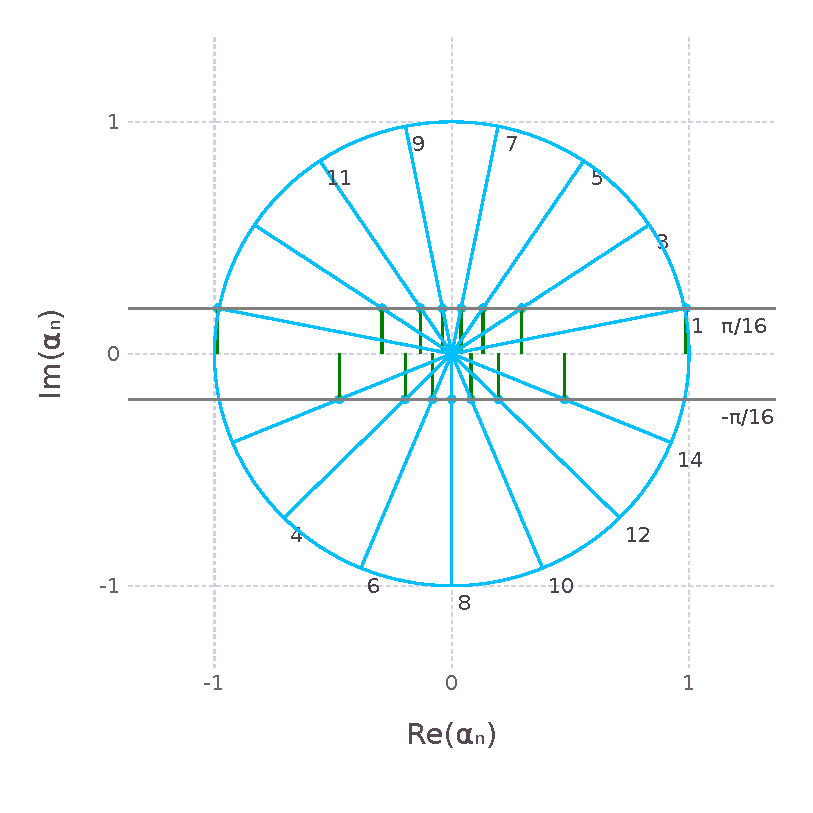
\includegraphics[natwidth=13cm,natheight=13cm]{pythagorean-16.pdf}
	\caption[Pythagorean coefficients for $p=16$]{Complex plane geometry of the Pythagorean coefficients $\alpha_n$ of period $p=16$. Blue points represent the location of the coefficients in the complex plane. Green lines illustrate the projection of the real component. Grey lines illustrate the imaginary component $\pm \frac{\pi}{16}$.}
	\label{fig:pythagorean-16}
\end{figure}
\begin{figure}[!ht]
	\centering
	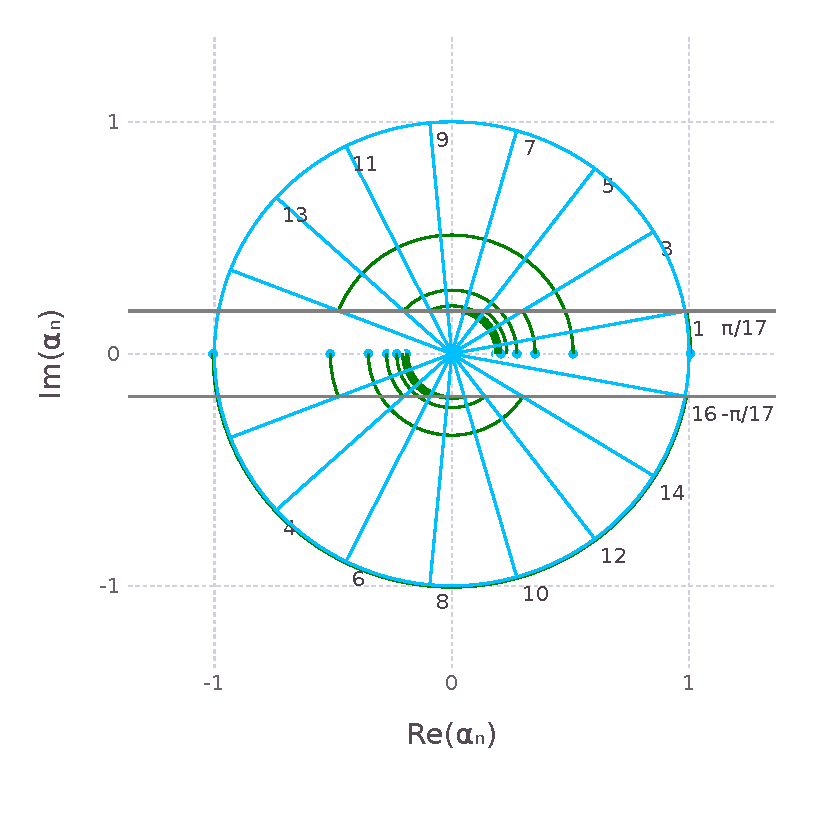
\includegraphics[natwidth=13cm,natheight=13cm]{pythagorean-17.pdf}
	\caption[Pythagorean coefficients for $p=17$]{Complex plane geometry of the Pythagorean coefficients $\alpha_n$ of period $p=17$. Blue points represent the location of the coefficients in the complex plane. Green lines carry the amplitude though to the intersection of the phase with the imaginary component $\pm \frac{\pi}{17}$.}
	\label{fig:pythagorean-17}
\end{figure}
	\chapter{Pad\'{e} Approximation of the Fr\'{e}chet Derivatives of the Exponential Map}
\section{The Gradient}
Moler and Van Loan seminally reviewed algorithms for calculating the matrix exponential in
1978, and revisited that review in 2003\cite{moler_nineteen_1978,moler_nineteen_2003}. 
Building on the discussions of Moler and Van Loan, Higham established the standard 
implementation of the matrix exponential based on scaling and scaring and Pad\'{e} 
approximation\cite{higham_scaling_2005,higham_functions_2008}. The Higham implementation was
further optimized for $64$ bit architectures by Al-Mohy\cite{al-mohy_new_2009}. In the same
work Al-Mohy developed an algorithm to approximate the derivative of the matrix exponential, 
formulated by taking the derivative of the Pad\'{e} approximation of the matrix exponential, 
and then working out a recursive calculation for the derivatives of matrix 
powers\cite{al-mohy_computing_2009}.

While the derivative of the Pad\'{e} approximation of an analytic function will converge to 
the derivative of the analytic function, it is not true that the derivative of the Pad\'{e} 
approximation of an analytic function is the Pad\'{e} approximation of the derivative of an 
analytic function. In the sense that Pad\'{e} approximations of analytic functions are an 
optimal series of algebraic approximations the 2009 method proposed by Al-Mohy is not 
optimal.

In this chapter we will develop an approximation for the first, and second order Fr\'{e}chet
derivatives of the matrix exponential, by decomposing the derivatives into components that
hold for the commutative condition, and components containing the perturbation due to 
non-commutativity. We will then derive the Pad\'{e} approximation for the non-commutative 
perturbation. We begin by listing the eight forms of the Fr\'{e}chet derivative of 
exponential map, in the direction $\frac{\partial X}{\partial x}$ at the point $X$ in the 
Lie algebra.
\footnote{We have abused and confounded the notations for directional derivatives and 
partial derivatives here by assuming that $X$ is parameterized by $x$ so that $\frac{\partial e^X}{\partial x}$
is the derivative in the direction of change of $x$.}
\footnote{With respect to the adjoint operator, we are using the currying partial 
application notation of $\left[L f\left(\cdotp\right)\right]\left(y\right)$ to indicate the 
application of the operator $L$ to $f\left(x\right)$ followed by evaluation of the result at
$y$.}
{\setlength{\IEEEnormaljot}{18pt}
\begin{IEEEeqnarray*}{rClls}
	\frac{\partial e^X}{\partial x}
		& = & e^X \left[\int_0^1 e^{- s\operatorname{ad}_{X} \cdotp} ds \right] \left(\frac{\partial X}{\partial x}\right) & & \\
		& = & e^X \left[\frac{1 - e^{-\operatorname{ad}_X \cdotp}}{\operatorname{ad}_X \cdotp}\right]\left(\frac{\partial X}{\partial x}\right) & \smash{\left. \IEEEstrut[4\jot] \right\rbrace} & \text{left recursive} \\
		& = & e^X \left[\sum_{n=0}^{\infty} \frac{\left(-1\right)^n}{\left(n+1\right)!} \operatorname{ad}_X^n \cdotp \right] \left(\frac{\partial X}{\partial x}\right) & & \\
		& = & \left[ \frac{\operatorname{ad}_{e^X} \cdotp}{\operatorname{ad}_X \cdotp} \right]\left(\frac{\partial X}{\partial x}\right) & & \text{adjoint ratio} \\
		& = & e^{\frac{1}{2}X} \left[ \frac{e^{\frac{1}{2}\operatorname{ad}_X \cdotp } - e^{-\frac{1}{2}\operatorname{ad}_X \cdotp}}{\operatorname{ad}_X \cdotp} \right]\left(\frac{\partial X}{\partial x}\right) e^{\frac{1}{2}X} & & \text{hyperbolic} \\
		& = & \left[ \int_0^1 e^{s \operatorname{ad}_{X} \cdotp} ds \right]\left(\frac{\partial X}{\partial x}\right) e^X & &\\
		& = & \left[ \frac{e^{\operatorname{ad}_X \cdotp} - 1}{\operatorname{ad}_X \cdotp} \right] \left(\frac{\partial X}{\partial x}\right) e^X & \smash{\left. \IEEEstrut[4\jot] \right\rbrace} & \text{right recursive}\\
		& = & \left[\sum_{n=0}^{\infty} \frac{1}{\left(n+1\right)!} \operatorname{ad}_X^n \cdotp \right] \left(\frac{\partial X}{\partial x} \right) e^X & &
\end{IEEEeqnarray*}}

The last equality demonstrates the non-commutative perturbation term most clearly; where the
first multiplicative factor in the derivative accounts for the lack of commutativity between
$X$ and $\frac{\partial X}{\partial x}$, and the last term resembles the derivative in the
commutative case. This can be seen clearly when considering the condition $\left[X,\frac{\partial X}{\partial x}\right]=0$ 
in which case $\frac{\partial e^X}{\partial x} = \frac{\partial X}{\partial x} e^X$. 

Even though the multiplicative factorization provides a transparent representation of the 
computational terms it is still far from optimal; because, when compared to matrix addition, 
matrix multiplication is both computationally more expensive, and less numerically stable. 
The numerical stability, and efficiency can be improved by decomposing the first 
multiplicative factor into a linear sum of the non-commutative perturbation term, which will 
reduce to $0$ when $\left[X,\frac{\partial X}{\partial x}\right]=0$, and an invariant term 
that contains the commutative relationship for all $X$.
\begin{IEEEeqnarray*}{rCl}
	\frac{\partial e^X}{\partial x}
		& = & \left[\frac{e^{\operatorname{ad}_X \cdotp} - 1 - \operatorname{ad}_X \cdotp }{\operatorname{ad}_X^2 \cdotp} \right] \left(\operatorname{ad}_X \frac{\partial X}{\partial x} \right) e^X + \frac{\partial X}{\partial x} e^X\\
		& = & \underbrace{\left[\sum_{n=0}^{\infty} \frac{1}{\left(n+2\right)!} \operatorname{ad}_X^n \cdotp \right] \left(\operatorname{ad}_X \frac{\partial X}{\partial x} \right)}_{\text{non-commutative anomaly}} e^X + \underbrace{\frac{\partial X}{\partial x}}_{\text{invariant}} e^X
\end{IEEEeqnarray*}

Formally the infinite series in the non-commutative perturbation is related to the lower 
incomplete gamma function $\gamma\left(n,x\right)$. This can be seen by considering the 
general case when the offset of $2$ in the factorial is allowed to be any natural number $n$, 
and then restating the sum in terms of a truncated exponential series.
\begin{IEEEeqnarray*}{rCl}
	\sum_{m=0}^{\infty} \frac{x^m}{\left(m+n\right)!}
		& = & \frac{1}{x^n} \sum_{m=n}^{\infty} \frac{x^m}{m!}\\
		& = & \frac{1}{x^n} \left(e^x - \sum_{m=0}^{n-1}\frac{x^m}{m!} \right)\\
		& = & \frac{1}{x^n} \left(e^x - e^x \frac{\Gamma\left(n,x\right)}{\Gamma\left(n\right)}\right)\\
		& = & \frac{e^x}{\left(n-1\right)! x^n} \left(\int_0^{\infty} t^{n-1}e^{-t}dt - \int_x t^{n-1} e^{-t}dt \right)\\
		& = & \frac{e^x}{\left(n-1\right)! x^n} \int_0^x t^{n-1}e^{-t}dt\\
		& = & \frac{e^x}{\left(n-1\right)! x^n} \gamma\left(n,x\right)
\end{IEEEeqnarray*}

The non-commutative perturbation series is linear in $\frac{\partial X}{\partial x}$  and a 
Taylor series in the powers of $\operatorname{ad}_X \cdotp$. Thus any computation of an 
approximation will be in the powers of $\operatorname{ad}_X \cdotp$. As was discussed in the 
Moler and Van Loan\cite{moler_nineteen_1978,moler_nineteen_2003}, naive computation of the 
Taylor series itself results in an approximation that will converge slowly, requiring a
larger number of powers to be computed before the threshold of floating point error is 
reached. Pad\'{e} approximation by rational functions remedy this problem, by offering 
convergence to the threshold of floating point error in smaller powers, and fewer 
computational steps.

However the question remains, given that $\frac{e^{x} -1 - x}{x^2}$ is a rational 
perturbation of $e^x$, why not simply reuse the polynomials of the Pad\'{e} approximation of 
the exponential function to compute new polynomials for a rational approximation of the 
non-commutative perturbation Taylor series. This method has two shortcomings: first, the 
approximation found in this manner is not itself a Pad\'{e} approximation of the anomaly 
Taylor series, and so is not bound by the same theoretical asymptotic results as Pad\'{e} 
approximations; second, computation by $\frac{e^{x} - 1 - x}{x^2}$ suffers from the same 
floating point errors near $0$ as naive computation of $e^x - 1$ by first computing $e^x$ 
and then subtracting $1$.

While it is clear that $\frac{e^x}{x^2}\gamma\left(2,x\right) : x \mapsto \frac{e^{x} -1 - x}{x^2}$ 
is analytic for $x \in \mathbb{R}$ or $x \in \mathbb{C}$, and thus can be approximated by a 
Pad\'{e} series with coefficients in $\mathbb{C}$; that the rational approximation with the 
same coefficients can be extended to $\operatorname{ad}_X \cdotp$ requires more careful 
consideration.

When $X$ is in $\mathfrak{st}(\hat{\mathbbm{1}})$ the adjoint operator $\operatorname{ad}_X \cdotp$
is a linear endomorphism on the vector space $\mathfrak{st}(\hat{\mathbbm{1}})$; and so 
belongs to the algebra of general linear operators $GL\left(\mathfrak{st}(\hat{\mathbbm{1}})\right)$. 
For a Pad\'{e} approximation with numerator polynomial $P\left(X\right)$ and denominator 
polynomial $Q\left(X\right)$, that $\operatorname{ad}_X \cdotp \in GL\left(\mathfrak{st}(\hat{\mathbbm{1}})\right)$
implies that $P\left(\operatorname{ad}_X \cdotp\right), Q\left(\operatorname{ad}_X \cdotp\right) \in GL\left(\mathfrak{st}(\hat{\mathbbm{1}})\right)$.
It follows that when a solution $Y$ to $\left[P\left(\operatorname{ad}_X \cdotp\right)\right] \left(\frac{\partial X}{\partial x}\right) = \left[Q\left(\operatorname{ad}_X \cdotp\right)\right] \left(Y\right) $
exists it is guaranteed to belong to $\mathfrak{st}(\hat{\mathbbm{1}})$, because $\frac{\partial X}{\partial x} \in \mathfrak{st}(\hat{\mathbbm{1}})$.

The remaining question is whether or not $Y$, a solution to $\left[P\left(\operatorname{ad}_X \cdotp\right)\right] \left(\frac{\partial X}{\partial x}\right) = \left[Q\left(\operatorname{ad}_X \cdotp\right)\right] \left(Y\right) $,
is an approximation of $\left[\sum_{n=0}^{\infty} \frac{1}{\left(n+2\right)!} \operatorname{ad}_X^n \cdotp \right] \left(\operatorname{ad}_X \frac{\partial X}{\partial x} \right)$?
Loosely, $\mathfrak{st}(\hat{\mathbbm{1}})$ is a normed vector space in the usual sense, so 
the convergence of the Pad\'{e} approximations that apply in scalar spaces carry over. Thus given
a sequence of Pad\'{e} approximations $Y_{mn}$ that solve $\left[P_n\left(\operatorname{ad}_X \cdotp\right)\right] \left(\frac{\partial X}{\partial x}\right) = \left[Q_m\left(\operatorname{ad}_X \cdotp\right)\right] \left(Y_{mn}\right) $,
we will converge $Y_{mn} \rightarrow \left[\sum_{n=0}^{\infty} \frac{1}{\left(n+2\right)!} \operatorname{ad}_X^n \cdotp \right] \left(\operatorname{ad}_X \frac{\partial X}{\partial x} \right)$.

Recapitulating $\left[n/m\right]_f\left(x\right)$ Pad\'{e} approximations, we seek a 
rational polynomial approximation to the Taylor series.
\begin{IEEEeqnarray*}{rCl}
	\frac{P_n\left(x\right)}{Q_m\left(x\right)}
		& =       & \frac{p_0 + p_1 x + \cdots + p_n x^n}{1 + q_1 x + \cdots + q_m x^m}\\
		& \approx & \sum_{n=0}^\infty \frac{1}{\left(n+2\right)!}x^n
\end{IEEEeqnarray*}

Such that the first $k \le n+m$ derivatives of the rational polynomial approximation evaluated at
$x=0$ equal the first $k \le n+m$ coefficients of the Taylor series.
\begin{IEEEeqnarray*}{rCl}
	\left.\frac{d^k}{d x^k}\frac{P_n\left(x\right)}{Q_m\left(x\right)}\right|_{x=0}
		& = & \frac{1}{\left(k+2\right)!}
\end{IEEEeqnarray*}

The symbolic computation of the exact rational coefficients of the $\left[13/14\right]_f\left(x\right)$ 
Pad\'{e} approximation was carried out in Julia programming language\cite{bezanson_julia:_2014}
using big integer mathematics, and the Polynomials package. The results of the computation 
are displayed in table \ref{tab:perturbation}. The order of the Pad\'{e} approximation 
was chosen so that the largest denominator in the rational coefficients of the numerator
polynomial $\left(7244400176133120000\right)$, and the largest denominator in the rational 
coefficients of the denominator polynomial $\left(6761440164390912000\right)$ were the 
largest integers less than the largest $64$ bit signed integer $\left(9223372036854775807\right)$.
This choice of approximation will need further research to better optimize.

To make use of the Pad\'{e} approximation we need to be able to compute powers of $\operatorname{ad}_X \cdotp$.
This can be accomplished through the Kronecker representation of $\operatorname{ad}_X \cdotp$, 
which requires representing the matrices of $\mathfrak{st}(\hat{\mathbbm{1}})$ as vectors. 
The vector representation of a matrix is achieved by the matrix reshaping  operator $\operatorname{vec}\left(Y\right) = \vec{y}$, 
which forms a vector $\vec{y}$ by concatenation of the columns of $Y$, called the 
vectorization of the matrix. We denote the inverse operator to vectorization $\operatorname{mat}\left(\vec{y}\right) = \operatorname{vec}^{-1}\left(\vec{y}\right) = Y$,
which reshapes a vector, of $n^2$ entries, into an $n \times n$ matrix.

After juggling the indexes of $\operatorname{vec}\left(\frac{\partial X}{\partial x}\right)$, 
the Kronecker representation of $\operatorname{ad}_X \frac{\partial X}{\partial x}$ follows
as
\begin{IEEEeqnarray*}{rCl}
	\operatorname{ad}_X \frac{\partial X}{\partial x} 
		& = & \operatorname{mat}\left( \left(I \otimes X - X^T \otimes I \right) \operatorname{vec}\left(\frac{\partial X}{\partial x}\right)\right)
\end{IEEEeqnarray*}

Proceeding by induction we find that 
\begin{IEEEeqnarray*}{rCl}
	\operatorname{ad}_X^n \frac{\partial X}{\partial x} 
		& = & \operatorname{mat}\left(\left(I \otimes X - X^T \otimes I \right)^n\operatorname{vec}\left(\frac{\partial X}{\partial x}\right)\right)
\end{IEEEeqnarray*}

It follows that $\frac{\partial e^X}{\partial x}$ can be computed by
\begin{IEEEeqnarray*}{rCl}
	\frac{\partial e^X}{\partial x}
		& = & \operatorname{mat}\left(\sum_{n=0}^{\infty} \frac{1}{\left(n+2\right)!} \left(I \otimes X - X^T \otimes I \right)^n \operatorname{vec}\left(\frac{\partial X}{\partial x}\right)\right) e^X + \frac{\partial X}{\partial x} e^X
\end{IEEEeqnarray*}

And thus can be approximated by
\begin{IEEEeqnarray*}{rCl}
	\frac{\partial e^X}{\partial x}
		& \approx & \operatorname{mat}\left(\frac{P_n\left(I \otimes X - X^T \otimes I\right)}{Q_m \left(I \otimes X - X^T \otimes I\right)} \operatorname{vec}\left(\frac{\partial X}{\partial x}\right) \right) e^X + \frac{\partial X}{\partial x} e^X
\end{IEEEeqnarray*}

We can summarize this work in an algorithm to compute the non-commutative perturbation\ref{alg:perturbation}.
This algorithm servers as a sketch only, highlighting only the novel elements developed in
this section. Many additional optimizations could be implemented including minimizing memory 
assignments by carrying out in place computations, conditioning matrices to improve
numerical stability, and using recursive squaring and summing methods to efficiently compute
the matrix polynomials. A point of concern is the first assignment of the Kronecker product, 
which results in a quadratic increase in the amount of memory used. Finally, an algorithm to 
compute the gradient of the matrix exponential can be formulated\ref{alg:gradient}.

\section{The Hessian}

Need preamble on combinatorics of powers of adjoint.
\begin{lemma}
	For any matrices $A,B$, differentiable matrix function $X$ parameterized by $x \in \mathbb{R}$, 
	and integer $n \ge 0$
	\begin{IEEEeqnarray*}{rCl}
		\left[\frac{\partial}{\partial x}\operatorname{ad}_X^n \cdot\right]\left( A\right)
			& = & \sum_{k=1}^n \left(\operatorname{ad}_X^{k-1} A \right)\left(\operatorname{ad}_{\frac{\partial X}{\partial x}} A\right)  \left(\operatorname{ad}_X^{n-k} A \right)\\
		\operatorname{ad}_X^n AB
			& = & \sum_{k=0}^n \binom{n}{k} \left(\operatorname{ad}_X^k A \right)\left(\operatorname{ad}_X^{n-k} B \right)\\
		\operatorname{ad}_X^n \left[A,B\right]
			& = & \sum_{k=0}^n \binom{n}{k} \left[\operatorname{ad}_X^k A , \operatorname{ad}_X^{n-k} B \right]
	\end{IEEEeqnarray*}
\end{lemma}

\begin{IEEEproof}
	For each of the equalities we have:
	\begin{enumerate}
		\item Proceed by induction on $n$.
		\item Proceed by induction on $n$.
		\item Take the antisymmetric difference of previous equality.\hfill\IEEEQEDhere
	\end{enumerate}
\end{IEEEproof}

We will also find use of the following corollary to the binomial theorem.
\begin{corollary}
	For any $n,m \ge 0$
	\begin{IEEEeqnarray*}{rCl}
		\sum_{k=m}^{n+m} \binom{k}{m}
			& = & \binom{n+m+1}{n}
	\end{IEEEeqnarray*}
\end{corollary}

\begin{IEEEproof}
	Proceed by induction on $n$.\hfill\IEEEQEDhere
\end{IEEEproof}

In the next step of developing the Hessian we derive the Taylor series for the bilinear 
non-commutative perturbation. Unfortunately because this form is a bilinear map it does
not admit the formulation of Pad\'{e} approximation.
\begin{corollary}
	For any differentiable matrix function $X$ parameterized by $x,y \in \mathbb{R}$
	\begin{IEEEeqnarray*}{rCl}
		\IEEEeqnarraymulticol{3}{l}
		{
			\left[\frac{\partial}{\partial x} \sum_{n=1}^\infty \frac{1}{\left(n+1\right)!} \operatorname{ad}_X^n \cdotp \right]\left(\frac{\partial X}{\partial y}\right)
			+ \left[\frac{\partial}{\partial y} \sum_{n=1}^\infty \frac{1}{\left(n+1\right)!} \operatorname{ad}_X^n \cdotp \right]\left(\frac{\partial Y}{\partial x}\right)
		}\\\quad
			& = & \sum_{n \ge m \ge 0} \frac{1}{\left(n+2\right)!} \left(\binom{n+1}{m+1} - \binom{n+1}{m} \right) \left[\operatorname{ad}_X^{m} \frac{\partial X}{\partial x} ,\operatorname{ad}_X^{n-m} \frac{\partial X}{\partial y} \right]
	\end{IEEEeqnarray*}
\end{corollary}

\begin{IEEEproof}
	Apply the previous results in the order they were stated to the symmetric sum of the two
	terms.
	\begin{IEEEeqnarray*}{rCl}
		\IEEEeqnarraymulticol{3}{l}
		{
			\left[\frac{\partial}{\partial x} \sum_{n=1}^\infty \frac{1}{\left(n+1\right)!} \operatorname{ad}_X^n \cdotp \right]\left(\frac{\partial X}{\partial y}\right)
			+ \left[\frac{\partial}{\partial y} \sum_{n=1}^\infty \frac{1}{\left(n+1\right)!} \operatorname{ad}_X^n \cdotp \right]\left(\frac{\partial Y}{\partial x}\right)
		}\\\quad
			& = & \sum_{n=1}^\infty \frac{1}{\left(n+1\right)!} \sum_{k=1}^n \operatorname{ad}_X^{k-1} \operatorname{ad}_{\frac{\partial X}{\partial x}} \operatorname{ad}_X^{n-k} \frac{\partial X}{\partial y}\\
			&   & +\: \sum_{n=1}^\infty \frac{1}{\left(n+1\right)!} \sum_{k=1}^n \operatorname{ad}_X^{k-1} \operatorname{ad}_{\frac{\partial X}{\partial y}} \operatorname{ad}_X^{n-k} \frac{\partial X}{\partial x}\\
			& = & \sum_{n=1}^\infty \frac{1}{\left(n+1\right)!} \sum_{k=1}^n \operatorname{ad}_X^{k-1} \left[ \frac{\partial X}{\partial x} ,\operatorname{ad}_X^{n-k} \frac{\partial X}{\partial y} \right]\\
			&   & +\: \sum_{n=1}^\infty \frac{1}{\left(n+1\right)!} \sum_{k=1}^n \operatorname{ad}_X^{k-1} \left[ \frac{\partial X}{\partial y} ,\operatorname{ad}_X^{n-k} \frac{\partial X}{\partial x} \right]\\
			& = & \sum_{n=1}^\infty \frac{1}{\left(n+1\right)!} \sum_{k=1}^n \sum_{m=0}^{k-1} \binom{k-1}{m} \left[\operatorname{ad}_X^{m} \frac{\partial X}{\partial x} ,\operatorname{ad}_X^{n-m-1} \frac{\partial X}{\partial y} \right]\\
			&   & +\: \sum_{n=1}^\infty \frac{1}{\left(n+1\right)!} \sum_{k=1}^n \sum_{m=0}^{k-1} \binom{k-1}{m} \left[\operatorname{ad}_X^{m} \frac{\partial X}{\partial y} ,\operatorname{ad}_X^{n-m-1} \frac{\partial X}{\partial x} \right]\\
			& = & \sum_{n=0}^\infty \frac{1}{\left(n+2\right)!} \sum_{k=0}^n \sum_{m=0}^{k} \binom{k}{m} \left[\operatorname{ad}_X^{m} \frac{\partial X}{\partial x} ,\operatorname{ad}_X^{n-m} \frac{\partial X}{\partial y} \right]\\
			&   & +\: \sum_{n=0}^\infty \frac{1}{\left(n+2\right)!} \sum_{k=0}^n \sum_{m=0}^{k} \binom{k}{m} \left[\operatorname{ad}_X^{m} \frac{\partial X}{\partial y} ,\operatorname{ad}_X^{n-m} \frac{\partial X}{\partial x} \right]\\
			& = & \sum_{n,m \ge 0}^\infty \frac{1}{\left(n+m+2\right)!} \left[\operatorname{ad}_X^{m} \frac{\partial X}{\partial x} ,\operatorname{ad}_X^{n} \frac{\partial X}{\partial y} \right] \sum_{k=m}^{n+m} \binom{k}{m}\\
			&   & +\: \sum_{n,m \ge 0}^\infty \frac{1}{\left(n+m+2\right)!} \left[\operatorname{ad}_X^{n} \frac{\partial X}{\partial y} ,\operatorname{ad}_X^{m} \frac{\partial X}{\partial x} \right] \sum_{k=n}^{n+m} \binom{k}{n}\\
			& = & \sum_{n,m \ge 0}^\infty \frac{1}{\left(n+m+2\right)!} \left(\binom{n+m+1}{n} - \binom{n+m+1}{m} \right) \left[\operatorname{ad}_X^{m} \frac{\partial X}{\partial x} ,\operatorname{ad}_X^{n} \frac{\partial X}{\partial y} \right]\\
			& = & \sum_{n \ge m \ge 0} \frac{1}{\left(n+2\right)!} \left(\binom{n+1}{m+1} - \binom{n+1}{m} \right) \left[\operatorname{ad}_X^{m} \frac{\partial X}{\partial x} ,\operatorname{ad}_X^{n-m} \frac{\partial X}{\partial y} \right]\\
			& = & \sum_{n=0}^\infty \frac{1}{\left(n+2\right)!} F_n
	\end{IEEEeqnarray*}
	Where we have defined $F_n$ recursively as:
	\begin{IEEEeqnarray*}{rCl}
		F_0 & = & 0\\
		F_{n+1} & = &  \left[\frac{\partial X}{\partial x},\operatorname{ad}_X^{n+1} \frac{\partial X}{\partial y}\right] + \operatorname{ad}_X F_n - \left[\operatorname{ad}_X^{n+1} \frac{\partial X}{\partial x},\frac{\partial X}{\partial y}\right]
	\end{IEEEeqnarray*}
	This recursive calculation is illustrate in figure \ref{fig:pascaldivergence}. The proof 
	of which is found by carrying out induction on $n$.\hfill\IEEEQEDhere
\end{IEEEproof}

There are three special cases that simplify the calculation of Taylor series considerably.
\begin{IEEEeqnarray*}{rCl}
	\sum_{n=0}^\infty \frac{ F_n}{\left(n+2\right)!}
	& = & 
		\begin{cases}
			0
				& \operatorname{ad}_X \frac{\partial X}{\partial x} = 0 \text{ and } \operatorname{ad}_X \frac{\partial X}{\partial y} = 0\\[1ex]
			\left[\frac{\partial X}{\partial x}, \sum_{n=0}^\infty \frac{n}{\left(n+2\right)!} \operatorname{ad}_X^n \frac{\partial X}{\partial y}\right]
				& \operatorname{ad}_X  \frac{\partial X}{\partial x} = 0\\[1ex]
			\left[\frac{\partial X}{\partial y}, \sum_{n=0}^\infty \frac{n}{\left(n+2\right)!} \operatorname{ad}_X^n \frac{\partial X}{\partial x}\right]
				& \operatorname{ad}_X  \frac{\partial X}{\partial y} = 0
		\end{cases}
\end{IEEEeqnarray*}

The Taylor series in the last two cases does admit a Pad\'{e} approximation, by the same
reasoning as presented in the previous section. In particular we can further reduce the
Taylor series.
\begin{IEEEeqnarray*}{rCl}
	\sum_{n=0}^\infty \frac{n}{\left(n+2\right)!} x^n
		& = & \sum_{n=1}^\infty \frac{n}{\left(n+2\right)!} x^n\\
		& = & \left(\sum_{n=0}^\infty \frac{n+1}{\left(n+3\right)!} x^n\right)x
\end{IEEEeqnarray*}

Using the same criteria as in the previous section yields a $\left[a/b\right]_f\left(x\right)$
Pad\'{e} approximation for $f\left(x\right) = \sum_{n=0}^\infty \frac{n+1}{\left(n+3\right)!} x^n$.
The coefficients of the Pad\'{e} approximation are summarized in table\ref{tab:bilinear}. 
This approximation is then used in a pair of branches in the calculation of the bilinear 
non-commutative perturbation to the Hessian\ref{alg:bilinear}.

Assuming that $\frac{\partial^2 X}{\partial x \partial y},\frac{\partial^2 X}{\partial y \partial x}$ 
are continuous we have, by corollary to Clairaut's theorem, that $\frac{\partial^2 e^X}{\partial x \partial y} = \frac{\partial^2 e^X}{\partial y \partial x}$.
We can then compute the Hessian by symmetrizing the partial differential so that 
antisymmetric terms cancel out.
\begin{IEEEeqnarray*}{rCl}
	\frac{1}{2} \left(\frac{\partial^2 e^X}{\partial x \partial y} + \frac{\partial^2 e^X}{\partial y \partial x}\right)
		& = & \frac{1}{2} \frac{\partial}{\partial x} \left[\sum_{n=0}^{\infty} \frac{1}{\left(n+1\right)!} \operatorname{ad}_X^n \cdotp \right] \left(\frac{\partial X}{\partial y} \right) e^X\\
		&   & +\: \frac{1}{2} \frac{\partial}{\partial y} \left[\sum_{n=0}^{\infty} \frac{1}{\left(n+1\right)!} \operatorname{ad}_X^n \cdotp \right] \left(\frac{\partial X}{\partial x} \right) e^X\\
		& = & \frac{1}{2} \left[\sum_{n=0}^{\infty} \frac{1}{\left(n+1\right)!} \operatorname{ad}_X^n \cdotp \right] \left(\frac{\partial X}{\partial y} \right) \left[\sum_{n=0}^{\infty} \frac{1}{\left(n+1\right)!} \operatorname{ad}_X^n \cdotp \right] \left(\frac{\partial X}{\partial x} \right) e^X\\
		&   & +\: \frac{1}{2} \left[\sum_{n=0}^{\infty} \frac{1}{\left(n+1\right)!} \operatorname{ad}_X^n \cdotp \right] \left(\frac{\partial^2 X}{\partial x \partial y} \right) e^X\\
		&   & \quad +\: \frac{1}{2} \left[ \frac{\partial}{\partial x} \sum_{n=0}^{\infty} \frac{1}{\left(n+1\right)!} \operatorname{ad}_X^n \cdotp \right] \left(\frac{\partial X}{\partial y}\right) e^X\\
		&   & +\: \frac{1}{2} \left[\sum_{n=0}^{\infty} \frac{1}{\left(n+1\right)!} \operatorname{ad}_X^n \cdotp \right] \left(\frac{\partial X}{\partial x} \right) \left[\sum_{n=0}^{\infty} \frac{1}{\left(n+1\right)!} \operatorname{ad}_X^n \cdotp \right] \left(\frac{\partial X}{\partial y} \right) e^X\\
		&   & \quad +\: \frac{1}{2} \left[\sum_{n=0}^{\infty} \frac{1}{\left(n+1\right)!} \operatorname{ad}_X^n \cdotp \right] \left(\frac{\partial^2 X}{\partial y \partial x} \right) e^X\\
		&   & \quad\quad +\: \frac{1}{2} \left[\frac{\partial}{\partial y} \sum_{n=0}^{\infty} \frac{1}{\left(n+1\right)!} \operatorname{ad}_X^n \cdotp \right] \left(\frac{\partial X}{\partial x}\right) e^X\\
		& = & \left[\sum_{n=0}^{\infty} \frac{1}{\left(n+1\right)!} \operatorname{ad}_X^n \cdotp \right] \left(\frac{\partial^2 X}{\partial x \partial y} \right) e^X\\
		&   & +\: \frac{1}{2} \left[\sum_{n=0}^{\infty} \frac{1}{\left(n+1\right)!} \operatorname{ad}_X^n \cdotp \right] \left(\frac{\partial X}{\partial y} \right) \left[\sum_{n=0}^{\infty} \frac{1}{\left(n+1\right)!} \operatorname{ad}_X^n \cdotp \right] \left(\frac{\partial X}{\partial x} \right) e^X\\
		&   & +\: \frac{1}{2} \left[\sum_{n=0}^{\infty} \frac{1}{\left(n+1\right)!} \operatorname{ad}_X^n \cdotp \right] \left(\frac{\partial X}{\partial x} \right) \left[\sum_{n=0}^{\infty} \frac{1}{\left(n+1\right)!} \operatorname{ad}_X^n \cdotp \right] \left(\frac{\partial X}{\partial y} \right) e^X\\
		&   & +\: \frac{1}{2} \sum_{n \ge m \ge 0} \frac{1}{\left(n+2\right)!} \left(\binom{n+1}{m+1} - \binom{n+1}{m} \right) \left[\operatorname{ad}_X^{m} \frac{\partial X}{\partial x} ,\operatorname{ad}_X^{n-m} \frac{\partial X}{\partial y} \right]
\end{IEEEeqnarray*}

The bilinear non-commutative perturbation is then called in the calculation of the Hessian
of the matrix exponential\ref{alg:hessian}.

\section{Figures and Illustrations}

\begin{longtable}{r r r}
	\caption{Pad\'{e} Approximation of $\sum_{n=0}^\infty \frac{1}{\left(n+2\right)!} x^n$}
	\label{tab:perturbation}\\
	\multicolumn{1}{l}{Degree} & \multicolumn{1}{l}{Numerator} & \multicolumn{1}{l}{Denominator}\\
	\hline
	\endfirsthead
	\caption*{Continued from previous page.}\\
	\multicolumn{1}{l}{Degree} & \multicolumn{1}{l}{Numerator} & \multicolumn{1}{l}{Denominator}\\
	\hline
	\endhead
	\caption*{Continued on next page.}
	\endfoot
	\caption*{The exact rational coefficients of the numerator and denominator polynomials of the $\left[ 13/14 \right]_f\left(x\right)$ Pad\'{e} approximation of $f\left(x\right)=\sum_{n=0}^\infty \frac{1}{\left(n+2\right)!} x^n$; symbolically computed.}
	\endlastfoot
	$x^{0}$ & $\frac{1}{2}$ & $\frac{1}{1}$\\
	$x^{1}$ & $\frac{-13}{174}$ & $\frac{-14}{29}$\\
	$x^{2}$ & $\frac{1}{58}$ & $\frac{13}{116}$\\
	$x^{3}$ & $\frac{-11}{7830}$ & $\frac{-13}{783}$\\
	$x^{4}$ & $\frac{11}{75168}$ & $\frac{11}{6264}$\\
	$x^{5}$ & $\frac{-11}{1461600}$ & $\frac{-11}{78300}$\\
	$x^{6}$ & $\frac{1}{2192400}$ & $\frac{11}{1252800}$\\
	$x^{7}$ & $\frac{-1}{64832400}$ & $\frac{-11}{25212600}$\\
	$x^{8}$ & $\frac{1}{1728864000}$ & $\frac{1}{57628800}$\\
	$x^{9}$ & $\frac{-1}{79873516800}$ & $\frac{-1}{1815307200}$\\
	$x^{10}$ & $\frac{1}{3594308256000}$ & $\frac{1}{72612288000}$\\
	$x^{11}$ & $\frac{-1}{295931379744000}$ & $\frac{-1}{3793992048000}$\\
	$x^{12}$ & $\frac{1}{28409412455424000}$ & $\frac{1}{273167427456000}$\\
	$x^{13}$ & $\frac{-1}{7244400176133120000}$ & $\frac{-1}{30185000733888000}$\\
	$x^{14}$ & & $\frac{1}{6761440164390912000}$
\end{longtable}

\begin{algorithm}
	\caption[Non-commutative Perturbation of $\frac{\partial e^X}{\partial x}$]{Numerical calculation the non-commutative perturbation of the gradient of the matrix exponential $\frac{\partial e^X}{\partial x}$.}
	\label{alg:perturbation}
	\begin{algorithmic}[1]
		\Function{PER}{$X$,$Dx$}
			\If{$\left[X,Dx\right] = 0$}
				\State $Y \gets 0$\Comment{Short circuit commutative case}
			\Else
				\State $adX \gets I \otimes X - X^T \otimes I$\Comment{if $X$ is $n \times n$ the result is $n^2 \times n^2$}
				\State $\vec{dx} \gets \operatorname{VEC}\left(Dx\right)$\Comment{Change of indexing}
				\State $P \gets P_{13}\left(adX\right)$\Comment{Recursive squaring and summing}
				\State $Q \gets Q_{14}\left(adX\right)$\Comment{Recursive squaring and summing}
				\State Solve for $\vec{y}$: $P \vec{dx} = Q \vec{y}$\Comment{Call to linear solver}
				\State $Y \gets \operatorname{MAT}\left(\vec{y}\right)$\Comment{Change of indexing}
			\EndIf
			\State \Return $Y$
		\EndFunction
	\end{algorithmic}
\end{algorithm}

\begin{algorithm}
	\caption[Gradient of $e^X$]{Numerical calculation of the gradient of the matrix exponential $\frac{\partial e^X}{\partial x}$.}
	\label{alg:gradient}
	\begin{algorithmic}[1]
		\Function{GEX}{$X$,$Dx$}
			\State $E \gets e^X$\Comment{Call to matrix exponential}
			\State $P \gets \operatorname{PER}\left(X,Dx\right)$\Comment{Call to non-commutative perturbation}
			\State \Return $\left(P + Dx\right) E$
		\EndFunction
	\end{algorithmic}
\end{algorithm}

\begin{figure}
	\centering
	\begin{tikzpicture}
		\node[text=gray] at (   0,   0) {$  0$};

		\node[text=gray] at (-1/2,  -1) {$  1$};
		\node[text=gray] at ( 1/2,  -1) {$ -1$};

		\node[text=gray] at (  -1,  -2) {$  1$};
		\node[font=\bf ] at (   0,  -2) {$  0$};
		\node[text=gray] at (   1,  -2) {$ -1$};

		\node[text=gray] at (-3/2,  -3) {$  1$};
		\node[font=\bf ] at (-1/2,  -3) {$  1$};
		\node[font=\bf ] at ( 1/2,  -3) {$ -1$};
		\node[text=gray] at ( 3/2,  -3) {$ -1$};

		\node[text=gray] at (  -2,  -4) {$  1$};
		\node[font=\bf ] at (  -1,  -4) {$  2$};
		\node[font=\bf ] at (   0,  -4) {$  0$};
		\node[font=\bf ] at (   1,  -4) {$ -2$};
		\node[text=gray] at (   2,  -4) {$ -1$};

		\node[text=gray] at (-5/2,  -5) {$  1$};
		\node[font=\bf ] at (-3/2,  -5) {$  3$};
		\node[font=\bf ] at (-1/2,  -5) {$  2$};
		\node[font=\bf ] at ( 1/2,  -5) {$ -2$};
		\node[font=\bf ] at ( 3/2,  -5) {$ -3$};
		\node[text=gray] at ( 5/2,  -5) {$ -1$};

		\node[text=gray] at (  -3,  -6) {$  1$};
		\node[font=\bf ] at (  -2,  -6) {$  4$};
		\node[font=\bf ] at (  -1,  -6) {$  5$};
		\node[font=\bf ] at (   0,  -6) {$  0$};
		\node[font=\bf ] at (   1,  -6) {$ -5$};
		\node[font=\bf ] at (   2,  -6) {$ -4$};
		\node[text=gray] at (   3,  -6) {$ -1$};

		\node[text=gray] at (-7/2,  -7) {$  1$};
		\node[font=\bf ] at (-5/2,  -7) {$  5$};
		\node[font=\bf ] at (-3/2,  -7) {$  9$};
		\node[font=\bf ] at (-1/2,  -7) {$  5$};
		\node[font=\bf ] at ( 1/2,  -7) {$ -5$};
		\node[font=\bf ] at ( 3/2,  -7) {$ -9$};
		\node[font=\bf ] at ( 5/2,  -7) {$ -5$};
		\node[text=gray] at ( 7/2,  -7) {$ -1$};

		\node[text=gray] at (  -4,  -8) {$  1$};
		\node[font=\bf ] at (  -3,  -8) {$  6$};
		\node[font=\bf ] at (  -2,  -8) {$ 14$};
		\node[font=\bf ] at (  -1,  -8) {$ 14$};
		\node[font=\bf ] at (   0,  -8) {$  0$};
		\node[font=\bf ] at (   1,  -8) {$-14$};
		\node[font=\bf ] at (   2,  -8) {$-14$};
		\node[font=\bf ] at (   3,  -8) {$ -6$};
		\node[text=gray] at (   4,  -8) {$ -1$};

		\node[text=gray] at (-9/2,  -9) {$  1$};
		\node[font=\bf ] at (-7/2,  -9) {$  7$};
		\node[font=\bf ] at (-5/2,  -9) {$ 20$};
		\node[font=\bf ] at (-3/2,  -9) {$ 28$};
		\node[font=\bf ] at (-1/2,  -9) {$ 14$};
		\node[font=\bf ] at ( 1/2,  -9) {$-14$};
		\node[font=\bf ] at ( 3/2,  -9) {$-28$};
		\node[font=\bf ] at ( 5/2,  -9) {$-20$};
		\node[font=\bf ] at ( 7/2,  -9) {$ -7$};
		\node[text=gray] at ( 9/2,  -9) {$ -1$};

		\node[text=gray] at (  -5, -10) {$\left[\frac{\partial X}{\partial x},\operatorname{ad}_X^{n+1} \frac{\partial X}{\partial y}\right]$};
		\node[text=gray] at (   5, -10) {$-\left[\operatorname{ad}_X^{n+1} \frac{\partial X}{\partial x},\frac{\partial X}{\partial y}\right]$};
	\end{tikzpicture}
	\caption[Pascal's triangle divergence]{Illustration of the calculation of the first 8 rows of coefficients of the divergence of Pascal's triangle; emphasizing the coefficients in $F_n$.}
	\label{fig:pascaldivergence}
\end{figure}

\begin{longtable}{r r r}
	\caption{Pad\'{e} Approximation of $\sum_{n=0}^\infty \frac{n+1}{\left(n+3\right)!} x^n$}
	\label{tab:bilinear}\\
	\multicolumn{1}{l}{Degree} & \multicolumn{1}{l}{Numerator} & \multicolumn{1}{l}{Denominator}\\
	\hline
	\endfirsthead
	\caption*{Continued from previous page.}\\
	\multicolumn{1}{l}{Degree} & \multicolumn{1}{l}{Numerator} & \multicolumn{1}{l}{Denominator}\\
	\hline
	\endhead
	\caption*{Continued on next page.}
	\endfoot
	\caption*{The exact rational coefficients of the numerator and denominator polynomials of the $\left[ a/b \right]_f\left(x\right)$ Pad\'{e} approximation of $f\left(x\right)=\sum_{n=0}^\infty \frac{n+1}{\left(n+3\right)!} x^n$; symbolically computed.}
	\endlastfoot
	$x^{0}$ & $\frac{1}{1}$ & $\frac{1}{1}$
\end{longtable}

\begin{algorithm}[!hb]
	\caption[Bilinear perturbation of $\frac{\partial^2 e^X}{\partial x \partial y}$]{Numerical calculation of the bilinear perturbation of the Hessian of the matrix exponential $\frac{\partial^2 e^X}{\partial x \partial y}$.}
	\label{alg:bilinear}
	\begin{algorithmic}[1]
		\Function{BIL}{$X$,$Dx$,$Dy$,$\epsilon = \text{machine float precision}$}
			\State $Ax \gets \left[X,Dx\right]$\Comment{Allocates memory}
			\State $Ay \gets \left[X,Dy\right]$\Comment{Allocates memory}
			\State $Z \gets 0$\Comment{Allocates memory}
			\If{$Ax \ne 0$ \textbf{and} $Ay \ne 0$}
				\State $F \gets \left[Dx, Ay\right] + \left[Dy,Ax\right]$\Comment{Allocates memory}
				\State $m \gets 3$\Comment{Factorial scalars}
				\State $n \gets 6$\Comment{Factorial scalars}
				\While{$ \left\| F \right\| > n\epsilon$}
					\State $Z \gets Z + \frac{F}{n}$\Comment{In place computation}
					\State $Ax \gets \left[X,Ax\right]$\Comment{In place computation}
					\State $Ay \gets \left[X,Ay\right]$\Comment{In place computation}
					\State $F \gets \left[Dx, Ay\right] + \left[X,F\right] + \left[Dx,Ax\right]$\Comment{In place computation}
					\State $m \gets m+1$\Comment{Increment factorial}
					\State $n \gets m n$\Comment{Increment factorial}
				\EndWhile
			\EndIf
			\State \Return $Z$
		\EndFunction
	\end{algorithmic}
\end{algorithm}

\begin{algorithm}[!hb]
	\caption[Hessian of $e^X$]{Numerical calculation of the Hessian of the matrix exponential $\frac{\partial^2 e^X}{\partial x \partial y}$.}
	\label{alg:hessian}
	\begin{algorithmic}[1]
		\Function{HEX}{$X$,$Dx$,$Dy$}
			\State \Return $Z$
		\EndFunction
	\end{algorithmic}
\end{algorithm}
	\chapter{Maximum Likelihood Estimation from First Hitting Times}
\section{Distribution of First Hitting Times}
Contemporary methods for fitting time homogeneous Markov processes on a finite 
state space require directly parameterizing the transition probability matrix $\mathbb{P}\left[X_n = j \left\|X_0 = i \right.\right] = \left\langle \hat{e}_i, P^n \hat{e}_j \right\rangle$,
as the methods depend on realizing the process through discrete time steps $n$. While this 
formulation has many powerful applications, there are analyses where the parameterization of 
the generator of the time homogeneous Markov process, $\mathbb{P}\left[X_t = j \left\|X_0 = i \right.\right] = \left\langle \hat{e}_i, \exp\left({tG}\right) \hat{e}_j \right\rangle$, 
is of greater meaning, or importance. In particular when the observed process is, at least
in principle, continuous or when the desired estimator is in units of rates per time, the 
parameterization of the generator is the more natural choice.

The natural experimental design for continuous time homogeneous Markov process on a
finite-state space is the observation of a stopped process, such as the statistic of the 
first hitting time to a state, or the first exit time from a state. Surprisingly, it is 
possible to explicitly formulate the distribution of these two statistics in terms of the 
generator of the process.

To start, recall the definition of the projection operator on a finite dimensional vector
space $P_i = \hat{e}_i \otimes \hat{e}_i$ which projects each vector in the space onto a
fixed unit vector $\hat{e}_i$. Projection operators hold a special purpose in analyzing
continuous time homogeneous Markov processes on finite-state spaces. The projection operator
$I-P_k$, when left multiplied to the generator $G = \sum_{ij}x_{ij}C_{ij}$, yields a new 
process $\left(I-P_k\right)G$, where state $k$ is an absorbing state.

The projection operators $P_i$ are useful in formulating the distribution of first hitting 
times of a process generated by $G$ in terms of the transition probabilities of a process
generated by $\left(I-P_i\right)G$. We can apply this to restate the first hitting time 
results in the exercises of Rogers and Williams \cite{rogers_diffusions_2000}.
\begin{theorem}
	If the statistic $T_k = \inf\left\lbrace t: X_t=k\right\rbrace$ is the first hitting time
	of the transition to state $k$ of a process generated by $G = \sum_{ij}x_{ij}C_{ij}$, then
	\begin{IEEEeqnarray*}{rCl}
		\mathbb{P}_G\left[T_k \le t \left\| X_0=l \right.\right]
			& = & 1 - \left\langle \hat{e}_l, \exp\left(t\left(I - P_k\right) G\right) \hat{e}_k \right\rangle.
	\end{IEEEeqnarray*}
\end{theorem}
\begin{IEEEproof}
	The proof hinges on formalizing the intuition that once we know a continuous time 
	homogeneous Markov process on a finite-state space $X_t$ has first touched the state $k$ 
	then we need no further information, and so we can work with the simpler process where $k$
	is an absorbing state. Being mindful to assure that every set is $\mathscr{F}_t$ 
	measurable, we calculate the cumulative distribution:
	\begin{IEEEeqnarray*}{+rCl+x*}
		\mathbb{P}_G\left[T_k \le t \left\| X_0=l \right.\right]
			& = & 1 - \mathbb{P}_G\left[T_k > t \left\| X_0=l \right.\right]\\
			& = & 1 - \mathbb{P}_G\left[\forall s \le t \enskip X_s \ne k, \enskip \exists u > t \enskip X_u=j \left\| X_0=l \right.\right]\\
			& = & 1 - \mathbb{P}_G\left[\forall s \le t \enskip X_s \ne k \left\| X_0=l \right.\right]\mathbb{P}_G\left[\exists u > t \enskip X_u=k \left\| \forall s \le t \enskip X_s \ne k \right.\right]\\
			& = & 1 - \mathbb{P}_G\left[\forall s \le t \enskip X_s \ne k \left\| X_0=l \right.\right]\mathbb{P}_G\left[X_u = k, u > t \left\| X_t \ne k \right.\right]\\
			& = & 1 - \mathbb{P}_{\left(I - P_k\right)G}\left[\forall s \le t \enskip X_s \ne k \left\| X_0=l \right.\right]\mathbb{P}_{\left(I - P_k\right)G}\left[X_u = k, \enskip u > t \left\| X_t \ne k \right.\right]\\
			& = & 1 - \mathbb{P}_{\left(I - P_k\right)G}\left[\forall s \le t \enskip X_s \ne k, \enskip X_u = k, \enskip u > t  \left\| X_0=l \right.\right]\\
			& = & 1 - \mathbb{P}_{\left(I - P_k\right)G}\left[X_t = k \left\| X_0=l \right.\right]\\
			& = & 1 - \left\langle \hat{e}_l, \exp\left(t\left(I - P_k\right) G\right) \hat{e}_k \right\rangle. & \IEEEQEDhere
	\end{IEEEeqnarray*}
\end{IEEEproof}
This result generalizes in a natural manner. To explain the generalization we will change 
notation slightly, eliding the explicit enumeration of states. Let $\hat{u} \ne \hat{v} \in \left\lbrace \hat{e}_1, \dots , \hat{e}_N \right\rbrace$
be a pair of distinct unit vectors representing states of the process, where $\hat{u}$ is 
the initial state, and $\hat{v}$ the final state with first hitting time statistic $T_{\hat{v}}$. 
Further, suppose we have additional data that the transition could only occur through any of
the allowed paths through states $\hat{u}_1, \dots \hat{u}_M \in \left\lbrace \hat{e}_1, \dots , \hat{e}_N \right\rbrace$
where all the unit vectors are pairwise unequal, i.e. $\hat{u}_k \ne \hat{u}, \hat{v}, \hat{u}_l$
for any $l \ne k$. The cumulative distribution of $T_{\hat{v}}$ is given by
\begin{IEEEeqnarray*}{rCl}
	\mathbb{P}_G\left[T_{\hat{v}} \le t \left\| X_0 = \hat{u} \right.\right]
		& = & 1 - \left\langle \hat{u}, \exp\left(t P G\right) \hat{v} \right\rangle.
\end{IEEEeqnarray*}
where the projection operator $P$ is over $\hat{u}$ and the allowed intermediate states
$\hat{u}_m$'s, i.e.
\begin{IEEEeqnarray*}{rCl}
	P
		& = & \hat{u} \otimes \hat{u}  + \sum_{m = 1}^M \hat{u}_m \otimes \hat{u}_m.
\end{IEEEeqnarray*}
This implies that if we can design our experiment to observe as many of the first hitting 
times as possible, and to minimize the number of unknown paths through intermediate states,
then we will greatly simplify our statistical estimators. In light of this, we can 
reformulate the standard textbook result, for example in Buchholz et. al \cite{buchholz_input_2014}, 
of the first hitting time statistic in the context of the stochastic contraction Lie algebra 
$\mathfrak{st}^{+}(\hat{\mathbbm{1}})$. As is standard we start with an experiment designed 
to observe the first hitting time statistic $T_j$ to state $\hat{e}_j$, from any other state 
$\hat{e_i}$ where $i \ne j$. Assuming the process is generated by $G = \sum_{ij}x_{ij}C_{ij}$ 
and keeping $i \ne j$ fixed, the density of $T_j$ is
\begin{IEEEeqnarray*}{rCl}
	p_G\left[T_j=t \left\| X_0=i \right.\right]
		& = & \frac{d}{dt} \mathbb{P}_G\left[ T_j\le t \left\| X_0=i \right.\right]\\
		& = & \frac{d}{dt} \mathbb{P}_{P_i G}\left[ T_j\le t \left\| X_0=i \right.\right]\\
		& = & \frac{d}{dt} \left(1 - \left\langle \hat{e}_i, \exp\left(tP_iG\right) \hat{e}_j\right) \right\rangle\\
		& = & \frac{d}{dt} \left(1 - \left\langle \hat{e}_i, \exp\left(t\sum_{l \ne i} x_{il} C_{il}\right) \hat{e}_j\right) \right\rangle\\
		& = & \frac{d}{dt} \left(1 - \left\langle \hat{e}_i, e^{-tx_{ij}} \hat{e}_i\right) \right\rangle\\
		& = & \frac{d}{dt} \left(1 - e^{-tx_{ij}}\right)\\
		& = & x_{ij} e^{-tx_{ij}}
\end{IEEEeqnarray*}
Intuitively if we design our experiment to observe the $N_{ij}$ replicated durations $t^{\left(n\right)} = T_j^{\left(n\right)}$
of every transition from $i$ to $j$, the maximum likelihood estimate of each rate, $x_{ij}$, 
is then the simple average
\begin{IEEEeqnarray*}{rCl}
	\tilde{x}_{ij}
		& = & \frac{N_{ij}}{\sum_{n=1}^{N_{ij}} t^{\left(n\right)}}
\end{IEEEeqnarray*}
However for experiments that involve an opportunistic sample, a survey, or a monitored 
population it is generally not possible to observe every distinct transition. Typically, the
initial state of the transition is known or can be inferred, but only a subset of states are
observed as absorbing, or exit states. In this situation the projection operator $P_i$ onto 
a single dimensional subspace is replaced with a projection $I - P_A = P_{i_1} + P_{i_2} + \cdots$ 
onto a multidimensional subspace, where $P_A$ is the projection onto the observed absorbing 
states in set $A$. In the next section we will name those states for which we can observe
absorption or exit as the sentinel states of the process.
\section{Likelihood and Its Maximization}
With a method to derive the density in hand we can proceed to formulate the log-likelihood
of first hitting time statistics. To do so we must carefully formulate the experimental 
design to which the log-likelihood will apply. Rather than attempting to formulate the 
possibly most general likelihood model possible, which would be notationally laborious given 
the infinite number of permutations and combinations of models available, we will illustrate 
the formulation of a log-likelihood through a specific application to an aging process.

An aging process is a continuous time homogeneous finite-state birth-death process where all 
the sequential transitions between states are reversible except for transitions to the final 
state, an absorbing state representing death. In the context of first hitting times, a 
finite subset of states act as sentinel states, where the first hitting time statistic for 
the transition between any pair of, possibly non-adjacent, sentinel states is observed. An 
example of this process is illustrated in figure \ref{fig:agingprocess}, which displays a 
seven-state aging process with three sentinel states. The transitions between states that 
are not sentinel are not directly observed but rather act as a type of memory register 
that broadens the centrality of the distribution of first hitting times.

Given an $U$-state aging process, the generator $G$ takes on the simple sequential form
\begin{IEEEeqnarray*}{rCl}
	G 
		& = & \sum_{u=1}^{U-1} x_{u\left(u+1\right)}C_{u\left(u+1\right)} 
			+ \sum_{u=2}^{U-1} x_{u\left(u-1\right)}C_{i\left(u-1\right)} \\
		& = & \sum_{u=1}^{U-1} x_{u\left(u+1\right)}\left(\hat{e}_u \otimes \hat{e}_{u+1} - \hat{e}_u \otimes \hat{e}_u\right)
			+ \sum_{u=2}^{U-1} x_{u\left(u-1\right)}\left(\hat{e}_u \otimes \hat{e}_{u-1} - \hat{e}_u \otimes \hat{e}_u\right)
\end{IEEEeqnarray*}
The $U$-state aging process has $2U-3$ unknown parameters, $x_{u\left(u+1\right)}$ for $1 \le u \le U-1$,
and $x_{u\left(u-1\right)}$ for $2 \le u \le U-1$, that are required to be estimated, for 
example by likelihood maximization. Of the $U$ states, a subset of $V \le U$ states are 
sentinel states denoted by $1 \le u_1 < \cdots u_V \le U$. We observe the first hitting time 
statistics for the transitions between the $V$ sentinel states.

Using the generalization of the theorem in previous section, the generators $G_v^\pm$ for
the observed first hitting time statistics $T_{u_{v \pm 1}}$ are given by 
\footnote{Note the careful application of signs $\pm$ whose order must correspond on both sides of the equation.}
\begin{IEEEeqnarray*}{rCl}
	G_v^\pm
		& = & \sum_{u=u_{v}}^{u_{v \pm 1} \mp 1} P_u G\\
		& = & \sum_{u=u_{v}}^{u_{v \pm 1} \mp 1} \left(\hat{e}_u \otimes \hat{e}_u\right) G\\
		& = & \sum_{u=u_{v}}^{u_{v \pm 1} \mp 1} x_{u \left(u-1\right)}C_{u \left(u-1\right)} + x_{u \left(u+1\right)}C_{u \left(u+1\right)}.
\end{IEEEeqnarray*}
The distribution density of $T_{u_{v \pm 1}}$ can be concisely stated as
\begin{IEEEeqnarray*}{rCl}
	p_G\left[T_{u_{v \pm 1}} = t \left\| X_0 = u_v \right.\right]
		& = & \left\langle \hat{e}_{u_v}, G_v^\pm \exp\left(t G_v^\pm \right) \hat{e}_{u_{v \pm 1}} \right\rangle\\
		& = & \left\langle x_{u_v\left(u_v+1\right)}\hat{e}_{u_v+1} + x_{u_v\left(u_v-1\right)}\hat{e}_{{u_v}-1}, \exp\left(t G_v^\pm \right) \hat{e}_{u_{v \pm 1}} \right\rangle\\
		&   & \:- \left\langle \left(x_{u_v\left(u_v+1\right)}+x_{u_v\left(u_v-1\right)}\right)\hat{e}_{u_v}, \exp\left(t G_v^\pm \right) \hat{e}_{u_{v \pm 1}} \right\rangle
\end{IEEEeqnarray*}
The next step is to formulate the log-likelihood. This requires establishing the observed
data, to do so we will again elide the explicit enumeration of the states so that we can
emphasize the enumeration of the observations. We will start be considering the general
first hitting time log-likelihood, and then specify the formulation for the aging process.

Consider $N$ observations of first hitting time statistics $T_{\hat{v}}^{\left(n\right)} = t^{\left(n\right)}$,
of transitions from state $\hat{u}^{\left(n\right)}$ to state $\hat{v}^{\left(n\right)}$,
the allowed states indicated by the projection $P^{\left(n\right)}$. The log-likelihood is
then the sum over the observations
\begin{IEEEeqnarray*}{rCl}
	\Lambda_G
		& = & \sum_{n=1}^N \ln p_G\left[ T_{\hat{v}}^{\left(n\right)} = t^{\left(n\right)} \left\| X_0 = \hat{u}^{\left(n\right)} \right.\right]\\
		& = & \sum_{n=1}^N \ln \left\langle \hat{u}^{\left(n\right)}, P^{\left(n\right)} G \exp\left(t^{\left(n\right)} P^{\left(n\right)} G\right) \hat{v}^{\left(n\right)} \right\rangle\\
		& = & \sum_{n=1}^N \ln \left\langle \hat{u}^{\left(n\right)}, G \exp\left(t^{\left(n\right)} P^{\left(n\right)} G\right) \hat{v}^{\left(n\right)} \right\rangle
\end{IEEEeqnarray*}
For an aging process, if $\hat{u}^{\left(n\right)} = \hat{e}_u$, we denote $\hat{u}_{+}^{\left(n\right)} = \hat{e}_{u+1}$,
$\hat{u}_{-}^{\left(n\right)} = \hat{e}_{u-1}$, $x_{+}^{\left(n\right)} = x_{u\left(u+1\right)}$,
$x_{-}^{\left(n\right)} = x_{u\left(u-1\right)}$, and $x^{\left(n\right)} = x_{+}^{\left(n\right)} + x_{-}^{\left(n\right)}$ the log-likelihood simplifies to
\begin{IEEEeqnarray*}{rCl}
	\Lambda_G
		& = & \sum_{n=1}^N \ln \left\langle x_{+}^{\left(n\right)} \hat{u}_{+}^{\left(n\right)} + x_{-}^{\left(n\right)} \hat{u}_{-}^{\left(n\right)} - x^{\left(n\right)} \hat{u}^{\left(n\right)},\exp\left(t^{\left(n\right)} P^{\left(n\right)} G\right) \hat{v}^{\left(n\right)} \right\rangle
\end{IEEEeqnarray*}
Maximization of the general model requires differentiation by each of the parameters $x_{ij}$.
To simplify we elide the index and denote the general choice of parameter $x$; which could
be any one of the parameters $x_{ij}$. We further elide the indexes of the canonical
generator so that $C_x = C_{ij}$. Partial differentiation of the log-likelihood is then
\begin{IEEEeqnarray*}{rCl}
	\frac{\partial \Lambda_G}{\partial x}
		& = & \sum_{n=1}^N \frac{\left\langle \hat{u}^{\left(n\right)}, \left(C_x \exp\left(t^{\left(n\right)} P^{\left(n\right)} G\right) + G \frac{\partial}{\partial x} \exp\left(t^{\left(n\right)} P^{\left(n\right)} G\right)\right) \hat{v}^{\left(n\right)} \right\rangle}
			{\left\langle \hat{u}^{\left(n\right)}, G \exp\left(t^{\left(n\right)} P^{\left(n\right)} G\right) \hat{v}^{\left(n\right)} \right\rangle}
\end{IEEEeqnarray*}
In the aging process $x$ can be one of $2U-3$ parameters $x_{k \Delta_k}$, with $\Delta _k = k \pm 1$.
Using the same notation as for the log-likelihood the partial derivative is
\footnote{Note the careful application of signs $\pm$ whose order must correspond on both sides of the equation.}
\footnote{Note that the indicator function $\mathbb{I}$ is with respect to the equivalence $\equiv$ and not equality $=$. The equivalence relation checks that the variable $x_\pm^{\left(n\right)}$ is the same one as the partial differential variable $x$. It can be informally read as ``is the same parameter as''.}
\begin{IEEEeqnarray*}{rCl}
	\frac{\partial \Lambda_G}{\partial x}
		& = & \sum_{n=1}^N  \frac{\mathbb{I}\left[x \equiv x^{\left(n\right)}_\pm \right] \left\langle \hat{u}_{\pm}^{\left(n\right)} - \hat{u}^{\left(n\right)},\exp\left(t^{\left(n\right)} P^{\left(n\right)} G\right) \hat{v}^{\left(n\right)} \right\rangle}
			{\left\langle x_{+}^{\left(n\right)} \hat{u}_{+}^{\left(n\right)} + x_{-}^{\left(n\right)} \hat{u}_{-}^{\left(n\right)} - x^{\left(n\right)} \hat{u}^{\left(n\right)},\exp\left(t^{\left(n\right)} P^{\left(n\right)} G\right) \hat{v}^{\left(n\right)} \right\rangle}\\
		&   & \:+ \frac{\left\langle x_{+}^{\left(n\right)} \hat{u}_{+}^{\left(n\right)} + x_{-}^{\left(n\right)} \hat{u}_{-}^{\left(n\right)} - x^{\left(n\right)} \hat{u}^{\left(n\right)},\frac{\partial}{\partial x} \exp\left(t^{\left(n\right)} P^{\left(n\right)} G\right) \hat{v}^{\left(n\right)} \right\rangle}
			{\left\langle x_{+}^{\left(n\right)} \hat{u}_{+}^{\left(n\right)} + x_{-}^{\left(n\right)} \hat{u}_{-}^{\left(n\right)} - x^{\left(n\right)} \hat{u}^{\left(n\right)},\exp\left(t^{\left(n\right)} P^{\left(n\right)} G\right) \hat{v}^{\left(n\right)} \right\rangle}
\end{IEEEeqnarray*}
Eliding the state enumerating indexes $i,j$ into the data enumerating index $n$ clarifies
the distinction between the provided data, and the parameters requiring estimation. Each 
individual summand in the first partial derivative of the log-likelihood requires the data: $t^{\left(n\right)}$ 
the observed time; $\hat{u}^{\left(n\right)}$ the observed initial state; $\hat{v}^{\left(n\right)}$ 
the observed final state; and $P^{\left(n\right)}$ the allowed intermediate states, 
including $\hat{u}^{\left(n\right)}$. A single summand in the partial derivative requires, 
$G$, the generator of the process as a parameter \ref{alg:singlesummand}.

For the aging process, given a single differential parameter $x_{k \Delta_k}$, we determine 
the canonical generator $C_{k \Delta_k}$, and then loop through the data computing the 
sub-generator $G_v^\pm$, which is supplied to the algorithm to compute the partial 
derivative of the matrix exponential. The terms are summed to produce the full partial 
derivative of the log-likelihood with respect to $x_{k \Delta_k}$ \ref{alg:completesum}. In 
the case of calculating all the partial derivatives of the log-likelihood, for large data 
sets it is more efficient to loop through the data once, calculating all the partial 
derivatives at each data point, and then producing the sum of the derivatives \ref{alg:allpartials}. 

While the gradient alone is sufficient for gradient decent searches for local maximum, the 
maximization of the log-likelihood by the Newton-Raphson method requires calculation of the
Hessian of the log-likelihood. By necessity the Hessian of the log-likelihood will be 
complicated. For the second partial derivative let $y$ be any single parameter $x_{ij}$, 
even possibly $x = y$, with $C_y$ elided equivalently; the second partial derivative is then
\begin{IEEEeqnarray*}{rCl}
	\frac{\partial^2 \Lambda_G}{\partial x \partial y}
		& = & \sum_{n=1}^N \frac{\left\langle \hat{u}^{\left(n\right)}, \left(C_x \frac{\partial}{\partial y} \exp\left(t^{\left(n\right)} P^{\left(n\right)} G\right) + C_y \frac{\partial}{\partial x} \exp\left(t^{\left(n\right)} P^{\left(n\right)} G\right)\right) \hat{v}^{\left(n\right)} \right\rangle}
			{\left\langle \hat{u}^{\left(n\right)}, G \exp\left(t^{\left(n\right)} P^{\left(n\right)} G\right) \hat{v}^{\left(n\right)} \right\rangle}\\
		&   & \:+ \frac{\left\langle \hat{u}^{\left(n\right)}, G \frac{\partial^2}{\partial x \partial y} \exp\left(t^{\left(n\right)} P^{\left(n\right)} G\right) \hat{v}^{\left(n\right)} \right\rangle}
			{\left\langle \hat{u}^{\left(n\right)}, G \exp\left(t^{\left(n\right)} P^{\left(n\right)} G\right) \hat{v}^{\left(n\right)} \right\rangle}\\
		&   & \:- \frac{\left\langle \hat{u}^{\left(n\right)}, \left(C_x \exp\left(t^{\left(n\right)} P^{\left(n\right)} G\right) + G \frac{\partial}{\partial x} \exp\left(t^{\left(n\right)} P^{\left(n\right)} G\right)\right) \hat{v}^{\left(n\right)} \right\rangle}
			{\left\langle \hat{u}^{\left(n\right)}, G \exp\left(t^{\left(n\right)} P^{\left(n\right)} G\right) \hat{v}^{\left(n\right)} \right\rangle}\\
		&   & \cdot \frac{\left\langle \hat{u}^{\left(n\right)}, \left(C_y \exp\left(t^{\left(n\right)} P^{\left(n\right)} G\right) + G \frac{\partial}{\partial y} \exp\left(t^{\left(n\right)} P^{\left(n\right)} G\right)\right) \hat{v}^{\left(n\right)} \right\rangle}
			{\left\langle \hat{u}^{\left(n\right)}, G \exp\left(t^{\left(n\right)} P^{\left(n\right)} G\right) \hat{v}^{\left(n\right)} \right\rangle}
\end{IEEEeqnarray*}
In our running example of the aging process, we have two simplifications at our disposal.
First, the generator $G$ is linear in $x_{ij}$ and so the second derivatives vanish. Second,
the partial derivative by the transition rates $x_{k \Delta_k }$ and $x_{l \Delta _l }$ will
only be non-trivial when the states fall between the same sentinel states
\footnote{Note the careful application of signs $\pm$ whose order must correspond on both sides of the equation.}
\footnote{Note that the indicator function $\mathbb{I}$ is with respect to the equivalence $\equiv$ and not equality $=$. The equivalence relation checks that the variable $x_\pm^{\left(n\right)}$ is the same one as the partial differential variable $x$. It can be informally read as ``is the same parameter as''.}
\begin{IEEEeqnarray*}{rCl}
	\frac{\partial^2 \Lambda_G}{\partial x \partial y}
		& = & \sum_{n=1}^N \frac{\mathbb{I}\left[x \equiv x^{\left(n\right)}_\pm \right] \left\langle \hat{u}_{\pm}^{\left(n\right)} - \hat{u}^{\left(n\right)}, \frac{\partial}{\partial y} \exp\left(t^{\left(n\right)} P^{\left(n\right)} G\right) \hat{v}^{\left(n\right)} \right\rangle}
			{\left\langle x_{+}^{\left(n\right)} \hat{u}_{+}^{\left(n\right)} + x_{-}^{\left(n\right)} \hat{u}_{-}^{\left(n\right)} - x^{\left(n\right)} \hat{u}^{\left(n\right)},\exp\left(t^{\left(n\right)} P^{\left(n\right)} G\right) \hat{v}^{\left(n\right)} \right\rangle}\\[2ex]
		&   & \:+ \frac{\mathbb{I}\left[y \equiv x^{\left(n\right)}_\pm \right] \left\langle \hat{u}_{\pm}^{\left(n\right)} - \hat{u}^{\left(n\right)}, \frac{\partial}{\partial x} \exp\left(t^{\left(n\right)} P^{\left(n\right)} G\right) \hat{v}^{\left(n\right)} \right\rangle}
			{\left\langle x_{+}^{\left(n\right)} \hat{u}_{+}^{\left(n\right)} + x_{-}^{\left(n\right)} \hat{u}_{-}^{\left(n\right)} - x^{\left(n\right)} \hat{u}^{\left(n\right)},\exp\left(t^{\left(n\right)} P^{\left(n\right)} G\right) \hat{v}^{\left(n\right)} \right\rangle}\\[2ex]
		&   & \:+ \frac{\left\langle x_{+}^{\left(n\right)} \hat{u}_{+}^{\left(n\right)} + x_{-}^{\left(n\right)} \hat{u}_{-}^{\left(n\right)} - x^{\left(n\right)} \hat{u}^{\left(n\right)},\frac{\partial^2}{\partial x \partial y} \exp\left(t^{\left(n\right)} P^{\left(n\right)} G\right) \hat{v}^{\left(n\right)} \right\rangle}
			{\left\langle x_{+}^{\left(n\right)} \hat{u}_{+}^{\left(n\right)} + x_{-}^{\left(n\right)} \hat{u}_{-}^{\left(n\right)} - x^{\left(n\right)} \hat{u}^{\left(n\right)},\exp\left(t^{\left(n\right)} P^{\left(n\right)} G\right) \hat{v}^{\left(n\right)} \right\rangle}\\[2ex]
		&   & \:- \left(\frac{\mathbb{I}\left[x \equiv x^{\left(n\right)}_\pm \right] \left\langle \hat{u}_{\pm}^{\left(n\right)} - \hat{u}^{\left(n\right)},\exp\left(t^{\left(n\right)} P^{\left(n\right)} G\right) \hat{v}^{\left(n\right)} \right\rangle}
			{\left\langle x_{+}^{\left(n\right)} \hat{u}_{+}^{\left(n\right)} + x_{-}^{\left(n\right)} \hat{u}_{-}^{\left(n\right)} - x^{\left(n\right)} \hat{u}^{\left(n\right)},\exp\left(t^{\left(n\right)} P^{\left(n\right)} G\right) \hat{v}^{\left(n\right)} \right\rangle}\right.\\[2ex]
		&   & \:+ \left. \frac{\left\langle x_{+}^{\left(n\right)} \hat{u}_{+}^{\left(n\right)} + x_{-}^{\left(n\right)} \hat{u}_{-}^{\left(n\right)} - x^{\left(n\right)} \hat{u}^{\left(n\right)},\frac{\partial}{\partial x} \exp\left(t^{\left(n\right)} P^{\left(n\right)} G\right) \hat{v}^{\left(n\right)} \right\rangle}
			{\left\langle x_{+}^{\left(n\right)} \hat{u}_{+}^{\left(n\right)} + x_{-}^{\left(n\right)} \hat{u}_{-}^{\left(n\right)} - x^{\left(n\right)} \hat{u}^{\left(n\right)},\exp\left(t^{\left(n\right)} P^{\left(n\right)} G\right) \hat{v}^{\left(n\right)} \right\rangle}\right)\\[2ex]
		&   & \cdot \left(\frac{\mathbb{I}\left[y \equiv x^{\left(n\right)}_\pm \right] \left\langle \hat{u}_{\pm}^{\left(n\right)} - \hat{u}^{\left(n\right)},\exp\left(t^{\left(n\right)} P^{\left(n\right)} G\right) \hat{v}^{\left(n\right)} \right\rangle}
			{\left\langle x_{+}^{\left(n\right)} \hat{u}_{+}^{\left(n\right)} + x_{-}^{\left(n\right)} \hat{u}_{-}^{\left(n\right)} - x^{\left(n\right)} \hat{u}^{\left(n\right)},\exp\left(t^{\left(n\right)} P^{\left(n\right)} G\right) \hat{v}^{\left(n\right)} \right\rangle}\right.\\[2ex]
		&   & \:+ \left. \frac{\left\langle x_{+}^{\left(n\right)} \hat{u}_{+}^{\left(n\right)} + x_{-}^{\left(n\right)} \hat{u}_{-}^{\left(n\right)} - x^{\left(n\right)} \hat{u}^{\left(n\right)},\frac{\partial}{\partial y} \exp\left(t^{\left(n\right)} P^{\left(n\right)} G\right) \hat{v}^{\left(n\right)} \right\rangle}
			{\left\langle x_{+}^{\left(n\right)} \hat{u}_{+}^{\left(n\right)} + x_{-}^{\left(n\right)} \hat{u}_{-}^{\left(n\right)} - x^{\left(n\right)} \hat{u}^{\left(n\right)},\exp\left(t^{\left(n\right)} P^{\left(n\right)} G\right) \hat{v}^{\left(n\right)} \right\rangle}\right)
\end{IEEEeqnarray*}
A full implementation of both the Hessian of the log-likelihood, and the Newton-Raphson 
method for likelihood maximization is complex undertaking \ref{alg:secondpartial}, but 
fundamentally is not intractable. The Newton-Raphson method, in the notation developed in
this chapter, calculates the $m+1$ estimation of $\tilde{G}^{\left(m+1\right)}$ as
\begin{IEEEeqnarray*}{rCl}
	\tilde{G}^{\left(m+1\right)}
		& = & \tilde{G}^{\left(m\right)} - \left[ \vec{\frac{\partial^2 \Lambda_G}{\partial G^2}} \right]_{G=\tilde{G}^{\left(m\right)}}^{-1} \left[ \vec{\frac{\partial \Lambda_G}{\partial G}} \right]_{G=\tilde{G}^{\left(m\right)}}
\end{IEEEeqnarray*}
where $\vec{\frac{\partial \Lambda_G}{\partial G}}$ is the Fr\'{e}chet gradient with respect to the generator $G$, and 
$\vec{\frac{\partial^2 \Lambda_G}{\partial G^2}}$ is the Fr\'{e}chet Hessian.

For the most part, successful implementation requires patience and diligence on the part of 
the developer, along with rigorous unit testing against known closed form solutions for the 
gradient and Hessian of the matrix exponential.
\clearpage
\section{Figures and Illustrations}
\begin{figure}[!ht]
	\centering
	\begin{tikzpicture}[->,thick,node distance=2cm]
		\node[state, very thick, font=\bf] (healthy)                                        {$1$};
		\node[state, draw=gray, text=gray] (healthy-improving) [right of=healthy]           {$2$};
		\node[state, draw=gray, text=gray] (healthy-worsening) [right of=healthy-improving] {$3$};
		\node[state, very thick, font=\bf] (treated)           [right of=healthy-worsening] {$4$};
		\node[state, draw=gray, text=gray] (treated-improving) [right of=treated]           {$5$};
		\node[state, draw=gray, text=gray] (treated-worsening) [right of=treated-improving] {$6$};
		\node[state, very thick, font=\bf] (death)             [right of=treated-worsening] {$7$};
		\path
			(healthy)           edge [loop left, very thick, font=\bf]  node         {$-x_{12}$}                     (healthy)
			(healthy)           edge [bend left, very thick, font=\bf]  node [above] {$x_{12}$}                      (healthy-improving)
			(healthy-improving) edge [bend left, very thick, font=\bf]  node [below] {$x_{21}$}                      (healthy)
			(healthy-improving) edge [loop below, draw=gray, text=gray] node         {$-\left(x_{21}+x_{23}\right)$} (healthy-improving)
			(healthy-improving) edge [bend left, draw=gray, text=gray]  node [above] {$x_{23}$}                      (healthy-worsening)
			(healthy-worsening) edge [bend left, draw=gray, text=gray]  node [below] {$x_{32}$}                      (healthy-improving)
			(healthy-worsening) edge [loop above, draw=gray, text=gray] node         {$-\left(x_{32}+x_{34}\right)$} (healthy-worsening)
			(healthy-worsening) edge [bend left, very thick, font=\bf]  node [above] {$x_{34}$}                      (treated)
			(treated)           edge [bend left, very thick, font=\bf]  node [below] {$x_{43}$}                      (healthy-worsening)
			(treated)           edge [loop below, very thick, font=\bf] node         {$-\left(x_{43}+x_{45}\right)$} (treated)
			(treated)           edge [bend left, very thick, font=\bf]  node [above] {$x_{45}$}                      (treated-improving)
			(treated-improving) edge [bend left, very thick, font=\bf]  node [below] {$x_{54}$}                      (treated)
			(treated-improving) edge [loop above, draw=gray, text=gray] node         {$-\left(x_{54}+x_{56}\right)$} (treated-improving)
			(treated-improving) edge [bend left, draw=gray, text=gray]  node [above] {$x_{56}$}                      (treated-worsening)
			(treated-worsening) edge [bend left, draw=gray, text=gray]  node [below] {$x_{65}$}                      (treated-improving)
			(treated-worsening) edge [loop below, draw=gray, text=gray] node         {$-\left(x_{65}+x_{67}\right)$} (treated-worsening)
			(treated-worsening) edge [very thick, font=\bf]             node [above] {$x_{67}$} (death);
	\end{tikzpicture}
	\caption[$7$ State Aging Process]{A representation of an aging process by a reversible $7$ state birth-death process, with $3$ sentinel states: healthy ($1$), care placement ($4$), and death ($7$). Each pair of intermediate states represents either a state of improving ($2$, $5$) or worsening ($3$, $6$) health.}
	\label{fig:agingprocess}
\end{figure}
\begin{algorithm}[!ht]
	\caption[Single summand of $\frac{\partial \Lambda}{\partial x_{k\left(k \pm 1\right)}}$]{Numerical calculation of a single summand in the gradient of the log-likelihood $\frac{\partial \Lambda}{\partial x_{k\left(k \pm 1\right)}}$ of the first hitting time statistic of an aging process. The inner products do not need full evaluation, rather by definition of the basis $\hat{e}_i$ the inner products select entries from the matrix by index.}
	\label{alg:singlesummand}
	\begin{algorithmic}[1]
		\Function{PLL}{$G$, $t$, $i$, $j$, $k$, $l$}
			\If{$\left|k - l\right| \ne 1$}
				\State \Return 0
			\EndIf
			\State $E \gets \operatorname{EXP}\left(t G\right)$\Comment{Call to matrix exponential}
			\State $C \gets \hat{e}_k \otimes \hat{e}_l - \hat{e}_k \otimes \hat{e}_k$\Comment{Canonical generator}
			\State $D \gets \left(C + \operatorname{PEX}\left(G, C\right)\right)E$\Comment{Call to gradient perturbation}
			\State $x_{+} \gets \left\langle \hat{e}_i , G \hat{e}_{i+1} \right\rangle$\Comment{Right transition rate}
			\State $x_{-} \gets \left\langle \hat{e}_i , G \hat{e}_{i-1} \right\rangle$\Comment{Left transition rate}
			\State $x_0 \gets -\left(x_{+} + x_{-}\right)$\Comment{Central transition rate}
			\If{$k = i$}
				\State $e_{+} \gets \left\langle \hat{e}_{i+1}, E \hat{e}_j \right\rangle$\Comment{Right probability}
				\State $e_0 \gets \left\langle \hat{e}_i, E \hat{e}_j \right\rangle$\Comment{Central probability}
				\State $e_{-} \gets \left\langle \hat{e}_{i-1}, E \hat{e}_j \right\rangle$\Comment{Left probability}
				\State \Return $\frac{e_{l-k} - e_0 + t \left(x_{+} \left\langle \hat{e}_{i+1}, D \hat{e}_j \right\rangle + x_{-} \left\langle \hat{e}_{i-1}, D \hat{e}_j \right\rangle + x_0 \left\langle \hat{e}_i, D \hat{e}_j \right\rangle\right)}{x_{+} e_{+} + x_{-}e_{-} + x_0 e_0}$
			\EndIf
			\State \Return $t \frac{ x_{+} \left\langle \hat{e}_{i+1}, D \hat{e}_j \right\rangle + x_{-} \left\langle \hat{e}_{i-1}, D \hat{e}_j \right\rangle + x_0 \left\langle \hat{e}_i, D \hat{e}_j \right\rangle}{x_{+} \left\langle \hat{e}_{i+1}, E \hat{e}_j \right\rangle + x_{-} \left\langle \hat{e}_{i-1}, E \hat{e}_j \right\rangle + x_0 \left\langle \hat{e}_i, E \hat{e}_j \right\rangle}$
		\EndFunction
	\end{algorithmic}
\end{algorithm}
\begin{algorithm}[!ht]
	\caption[Complete sum of $\frac{\partial \Lambda}{\partial x_{kl}}$]{Numerical calculation of the gradient of the complete sum log-likelihood $\frac{\partial \Lambda}{\partial x_{kl}}$ of $M$ first hitting time statistics, for any  generator $G$. Implemented as a straight forward single instruction, multiple data loop (SIMD). The Kronecker product does not need to be computed as it represents matrix element assignment by index.  The supplied data includes the projection matrix $P$ that defines the states allowed along the path of transition. In the context of an aging process the projection is given by $P = \sum_{n=i \wedge j+1}^{i \vee j-1} \hat{e}_n \otimes \hat{e}_n$.}
	\label{alg:completesum}
	\begin{algorithmic}[1]
		\Function{CLL}{$G$, $\left\lbrace \left(t, i, j, P \right)_1 , \dots , \left(t, i, j, P \right)_M \right\rbrace$, $k$, $l$}
			\State $r \gets 0$\Comment{Loop initialization}
			\ForAll{$\left(t,i,j\right) \in \left\lbrace \left(t , i, j, P \right)_1 , \dots , \left(t, i, j, P \right)_M \right\rbrace$}
				\State $r \gets r + \operatorname{PLL}\left(PG, t, i, j, k, l\right)$ \Comment{SIMD computation}
			\EndFor
			\State \Return $r$
		\EndFunction
	\end{algorithmic}
\end{algorithm}
\begin{algorithm}[!ht]
	\caption[All partial derivatives of $\frac{\partial \Lambda}{\partial x_{kl}}$]{Numerical calculation of the every partial derivative of the  gradient of the complete sum log-likelihood $\frac{\partial \Lambda}{\partial x_{kl}}$ of $M$ first hitting time statistics, for any $N \times N$ generator $G$. Implemented as an iteration over the partial derivatives within a SIMD loop over the data. The Kronecker product does not need to be computed as it represents matrix element assignment by index. The supplied data includes the projection matrix $P$ that defines the states allowed along the path of transition. In the context of an aging process the projection is given by $P = \sum_{n=i \wedge j+1}^{i \vee j-1} \hat{e}_n \otimes \hat{e}_n$.}
	\label{alg:allpartials}
	\begin{algorithmic}[1]
		\Function{GLL}{$G$, $\left\lbrace \left(t, i, j, P \right)_1 , \dots , \left(t, i, j, P \right)_M \right\rbrace$}
			\State $R \gets 0$\Comment{Loop initialization}
			\ForAll{$\left(t,i,j\right) \in \left\lbrace \left(t , i, j, P \right)_1 , \dots , \left(t, i, j, P \right)_M \right\rbrace$}
				\State $G_v \gets PG$\Comment{First hitting time generator}
				\ForAll{$ k \in \left\lbrace i \wedge j+1, \dots , i \vee j-1 \right\rbrace $}
					\ForAll{$l \in \left\lbrace 1, \dots, N \right\rbrace$}
						\State $R \gets R + \operatorname{PLL}\left(G_v, t, i, j, k, l\right) \left(\hat{e}_k \otimes \hat{e}_l\right)$\Comment{SIMD computation}
					\EndFor
				\EndFor
			\EndFor
			\State \Return $R$
		\EndFunction
	\end{algorithmic}
\end{algorithm}
\begin{algorithm}[!ht]
	\caption[Single summand in $\frac{\partial^2 \Lambda}{\partial x_{k \Delta_k} \partial x_{l \Delta_l}}$]{Numerical calculation of a single summand in the Hessian of the log-likelihood $\frac{\partial^2 \Lambda}{\partial x_{k \Delta_k} \partial x_{l \Delta_l}}$ of a first hitting time statistics. The inner products do not need full evaluation, rather by definition of the basis $\hat{e}_i$ the inner products select entries from the matrix by index.}
	\label{alg:secondpartial}
	\begin{algorithmic}[1]
		\Function{PPL}{$G$, $t$, $i$, $j$, $k$, $\Delta_k$, $l$, $\Delta_l$}
			\State $E \gets \operatorname{EXP}\left(tG\right)$\Comment{Call to matrix exponential}
			\State $C_k \gets \hat{e}_k \otimes \hat{e}_{\Delta_k} - \hat{e}_k \otimes \hat{e}_k$\Comment{Canonical generator}
			\State $C_k \gets \hat{e}_l \otimes \hat{e}_{\Delta_l} - \hat{e}_l \otimes \hat{e}_l$\Comment{Canonical generator}
			\State $P_k \gets \left(C_k + \operatorname{PEX}\left(G,C_k\right)\right)$\Comment{Call to gradient perturbation}
			\State $P_l \gets \left(C_l + \operatorname{PEX}\left(G,C_l\right)\right)$\Comment{Call gradient perturbation}
			\State $x_{+} \gets \left\langle \hat{e}_i , G \hat{e}_{i+1} \right\rangle$\Comment{Right transition rate}
			\State $x_{-} \gets \left\langle \hat{e}_i , G \hat{e}_{i-1} \right\rangle$\Comment{Left transition rate}
			\State $x_0 \gets -\left(x_{+} + x_{-}\right)$\Comment{Central transition rate}
			\If{$k=i$}
				\State $e_{+} \gets \left\langle \hat{e}_{i+1}, t P_k E \hat{e}_j \right\rangle$\Comment{Right probability}
				\State $e_0 \gets \left\langle \hat{e}_i, t P_k E \hat{e}_j \right\rangle$\Comment{Central probability}
				\State $e_{-} \gets \left\langle \hat{e}_{i-1}, t P_k E \hat{e}_j \right\rangle$\Comment{Left probability}
				\State $e_k \gets e_{\Delta_k - k} - e_0 $
			\Else
				\State $e_k \gets 0$
			\EndIf
			\If{$l=i$}
				\State $e_{+} \gets \left\langle \hat{e}_{i+1}, t P_l E \hat{e}_j \right\rangle$\Comment{Right probability}
				\State $e_0 \gets \left\langle \hat{e}_i, t P_l E \hat{e}_j \right\rangle$\Comment{Central probability}
				\State $e_{-} \gets \left\langle \hat{e}_{i-1}, t P_l E \hat{e}_j \right\rangle$\Comment{Left probability}
				\State $e_l \gets e_{\Delta_l - l} - e_0$
			\Else
				\State $e_l \gets 0$
			\EndIf
			\State $p_{kl} \gets \left\langle \hat{e}_i, \frac{1}{2}\left(t \operatorname{BEX}\left(G,C_k,C_l\right) +  t^2 \left(P_k P_l + P_l P_k\right)\right) E \hat{e}_j \right\rangle$
			\State $p_k \gets PLL\left(G,t,i,j,k,\Delta_k\right)$\Comment{Call to single summand partial}
			\State $p_l \gets PLL\left(G,t,i,j,l,\Delta_l\right)$\Comment{Call to single summand partial}
			\State \Return $\frac{e_k+e_l+p_{kl}}{x_{+} \left\langle \hat{e}_{i+1}, E \hat{e}_j \right\rangle + x_{-} \left\langle \hat{e}_{i-1}, E \hat{e}_j \right\rangle + x_0 \left\langle \hat{e}_i, E \hat{e}_j \right\rangle}-p_k p_l$
		\EndFunction
	\end{algorithmic}
\end{algorithm}
	\chapter{Conclusion}
\section{Summary of Results}
In chapter two we reversed the normal development of stochastic matrices; which usually
starts with characterizing matrices as having non-negative entries with fixed row sums in a
standard orthonormal basis $\hat{e}_i$. The line of typical development then notices that
the vector $\vec{\mathbbm{1}} = \sum_{i=1}^n \hat{e}_i$ is an Eigenvector. Instead we began
by characterizing all invertible matrices $A$ such that $A \hat{\mathbbm{1}} = \hat{\mathbbm{1}}$
with respect to a fixed unit vector $\hat{\mathbbm{1}}$. We showed that there is always a 
basis $\hat{e}_i$ such that $\vec{\mathbbm{1}} = \sqrt{n} \hat{\mathbbm{1}}$ can be
interpreted as the row sum vector, and found that this allowed us to characterize both the Lie 
group in which the matrices $A \hat{\mathbbm{1}} = \hat{\mathbbm{1}}$ reside, and the Lie
algebra of tangents to the Lie group. We denoted the $St(\hat{\mathbbm{1}})$ stochastic Lie
group with respect to $\hat{\mathbbm{1}}$, and $\mathfrak{st}(\hat{\mathbbm{1}})$ the
stochastic Lie algebra with respect to $\hat{\mathbbm{1}}$. We further characterized the
doubly stochastic Lie group and algebra with respect to $\hat{\mathbbm{1}}$, respectively 
denoted $St(\hat{\mathbbm{1}}, \hat{\mathbbm{1}})$ and $\mathfrak{st}(\hat{\mathbbm{1}}, \hat{\mathbbm{1}})$,
of invertible matrices of fixed row and column sums with respect to $\hat{\mathbbm{1}}$. 
This accomplished by generalizing the stochastic Lie group and algebra to the dual
stochastic Lie group and algebra, $St^\dagger(\hat{\mathbbm{1}})$ and $\mathfrak{st}^dagger(\hat{\mathbbm{1}})$, 
of invertible matrices such that $A^\dagger \hat{\mathbbm{1}} = \hat{\mathbbm{1}}$.

In chapter three we used analytic and closure properties of the stochastic Lie algebras to
argue that the algorithms developed for calculating the gradient and Hessian of the matrix
exponential will result in matrices that belong to the stochastic Lie algebra. An initial
computation of the coefficients for a Pad\'{e} approximation was presented, and an sketch
of algorithms to calculate the gradient and the Hessian were outlined.

In chapter four we combined the results of the previous two chapters, illustrated through
the example of the aging process. The algorithms to calculate the log-likelihood, its
gradient, and Hessian were developed. Finally the Newton-Raphson maximization was briefly
introduced.
\section{Discussion}
Any attempt to fit the generator of a Markov process to observations is in essence an 
exercise in calculating the logarithm of a matrix. Like the scalar complex logarithm the
matrix logarithm is not unique, and has many branches. To demonstrate this point in chapter
two a calculation of one of the branches of the logarithm of permutations was developed, in
the context of the stochastic Lie algebra. However, much as there is a unique real logarithm
of a positive real number, working within the normal subgroup, and real the sub-algebra, of
the stochastic Lie group does provide for certain guarantees of algebraic and analytic
closure.


Application of Lie Theory to the embedding problem for first hitting times...
Differentiate between problem of choosing a branch of the matrix logarithm
and multiple Markov models having the same first hitting time distribution.
Once a principle branch of the logarithm is fixed stochastic Lie algebra can 
give meaning to the idea of a simplest model, the one expressed in the fewest 
canonical generators.

Pad\'{e} approximation needs optimization. The Kronecker vectorization means 
only low to moderate dimensional models can be handled, due to the quadratic
scaling.
	\bibliography{project-bibliography} 
	\bibliographystyle{amsplain}
	\appendix
	\chapter{Julia Implementations}
Basic implementations of the algorithms presented in Julia.

\begin{lstlisting}[language=Julia,caption=Poor man's symbolic computation of the Pade coefficients of the generalized hyperbolic functions in Julia]
# The polynomials package provides both the polynomial type and
# the Pade approximation algorithm. If it is not installed 
# uncomment the next line
# Pkg.add('Polynomials')
using('Polynomials')

# General function to compute the [n/m] approximation of
# 1 / (a k + b)!
f(n,m,a,b) = Pade
(
	Poly
	(
		[Rational(1,factorial(BigInt(a*k+b))) for k=0:(n+m+1)]
	),
	n,
	m
)

# Compute the desired coefficients
c = f(16,16,1,2)

# Print the numerator coefficients
c.p.a

# Print the denominator coefficients
c.q.a
\end{lstlisting}

\begin{lstlisting}[language=Julia,caption=An unoptimized implementation of gradient of the matrix exponential in Julia]
function dexpm(X,DX)
	# Check for commutation
	if X * DX = DX * X
		DX * expm(X)
		
	# Use the Pade coefficients to compute dexpm
	else
	end
end
\end{lstlisting}

\end{document}